
\newcommand{\figcollation}{%
\begin{figure*}[!t]
\centering
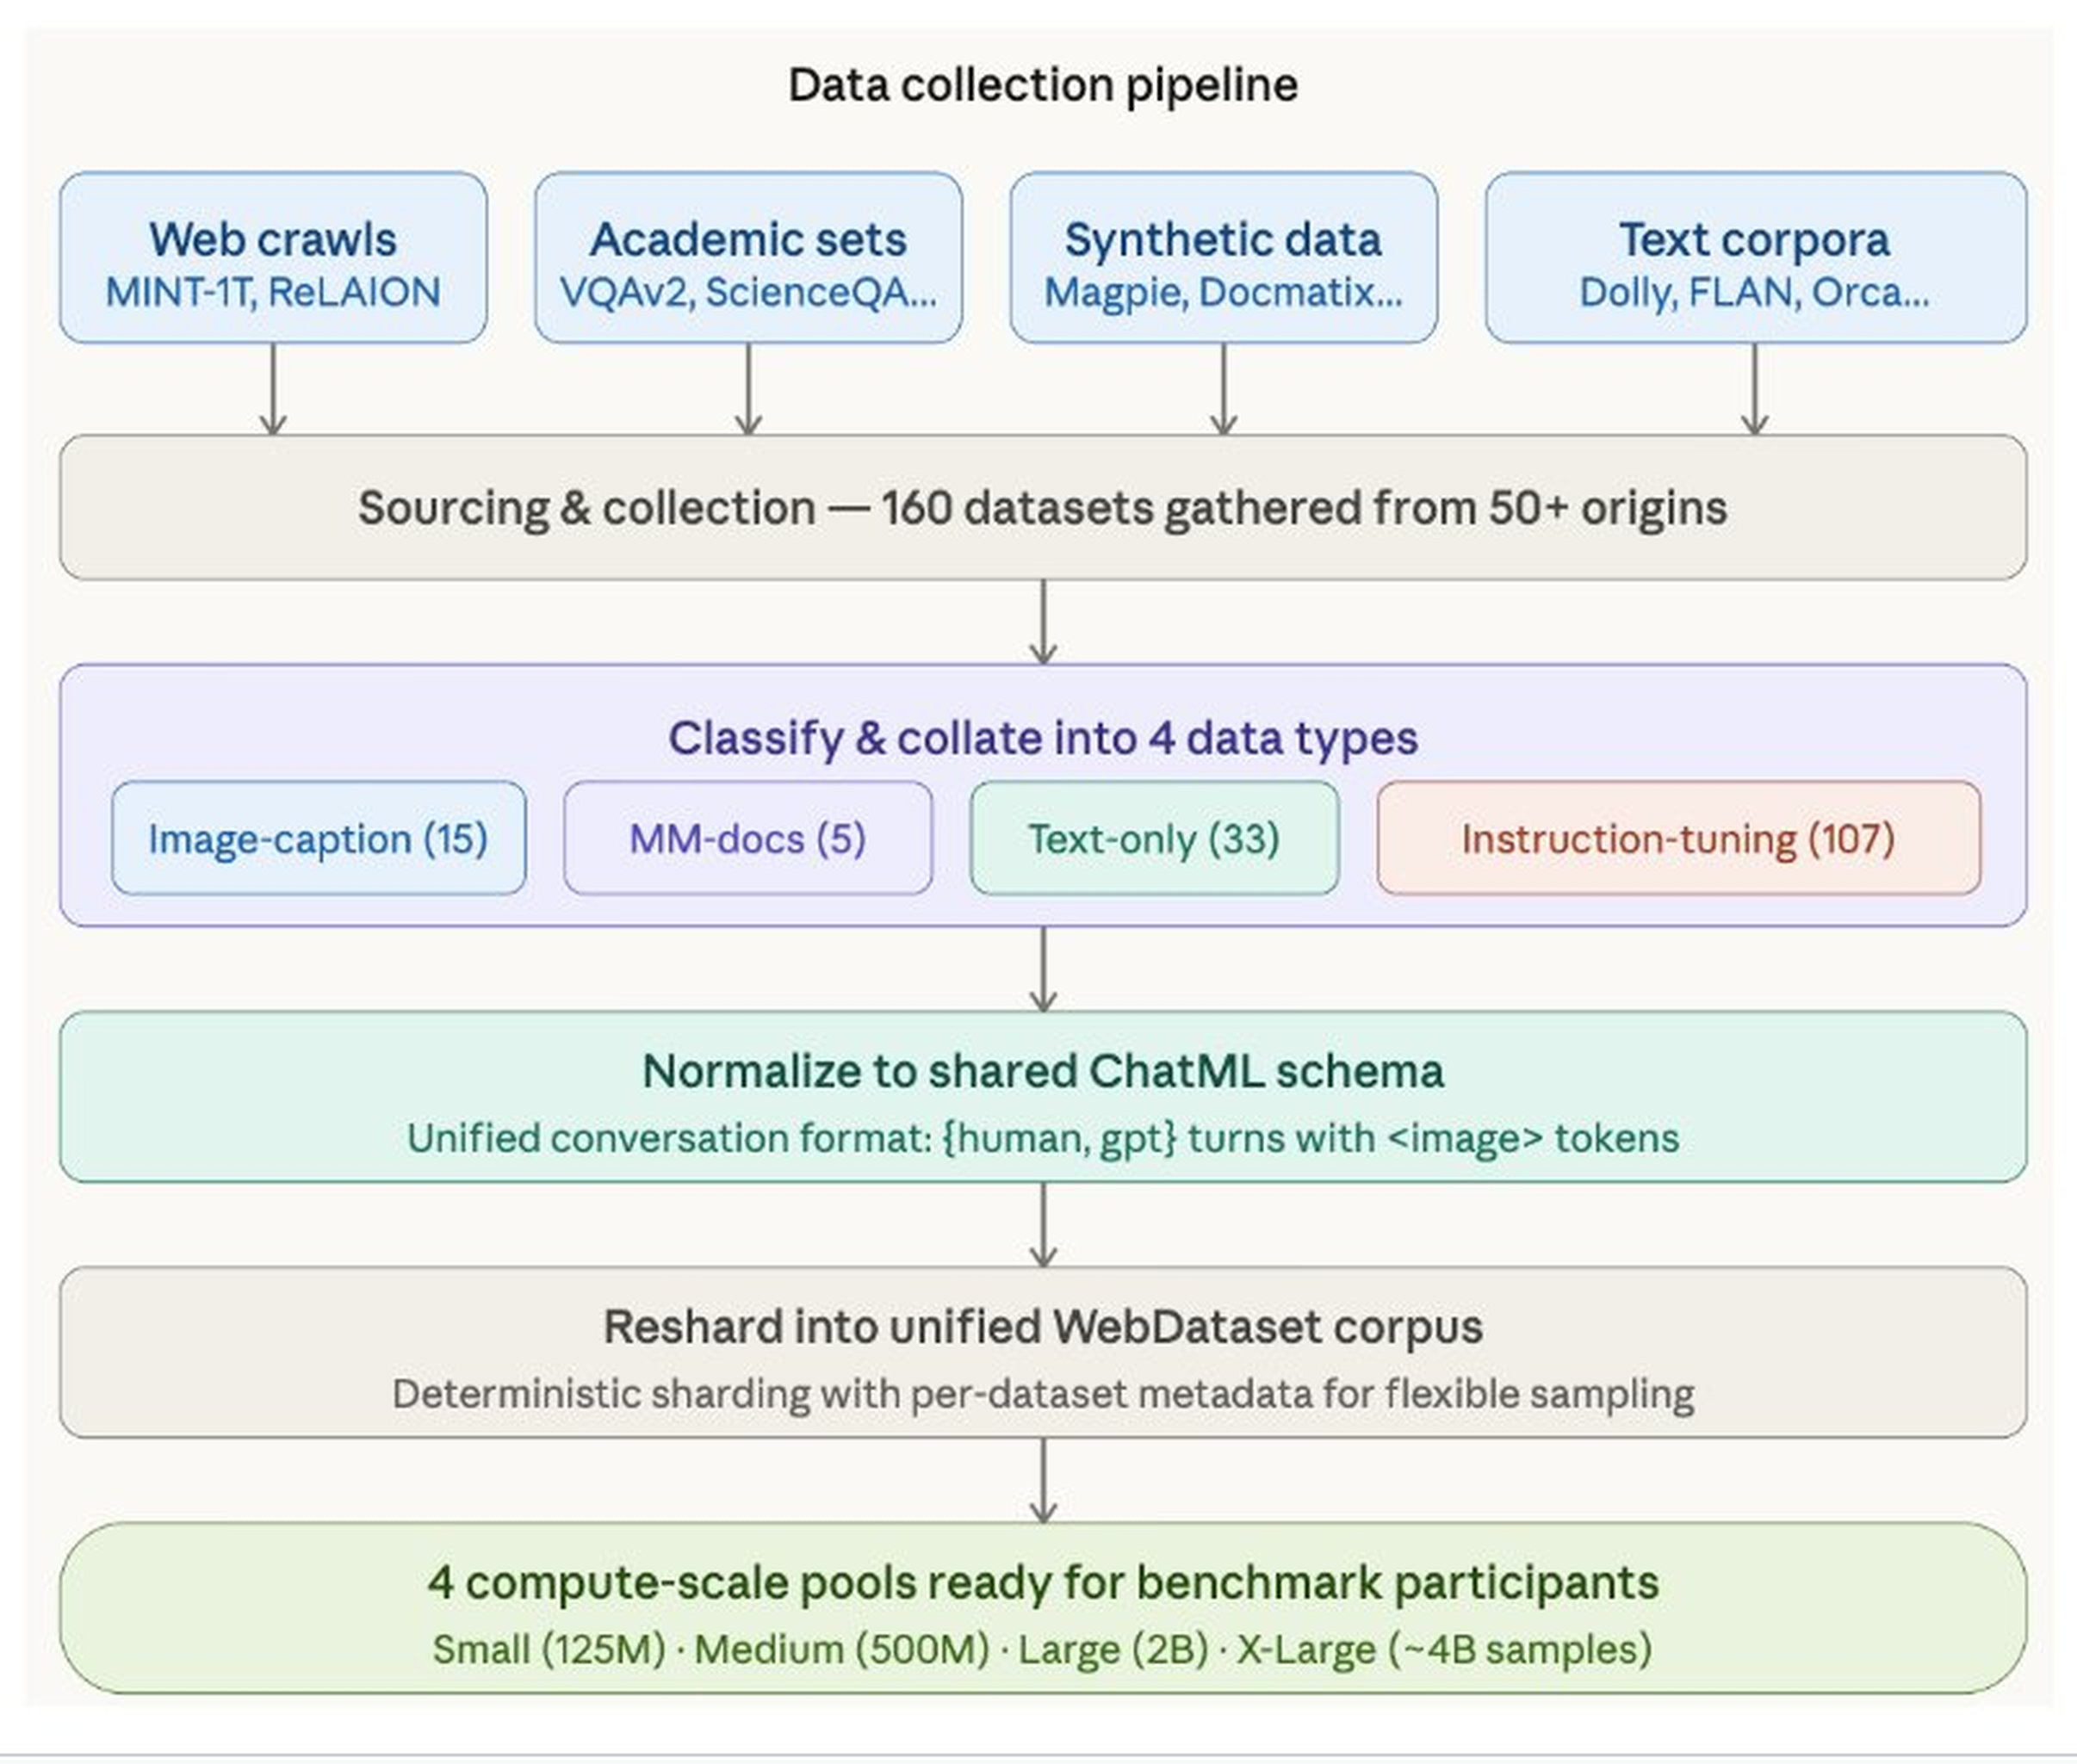
\includegraphics[width=0.8\linewidth]{figures/fig_data_collection_pipeline.png}
\caption{\textbf{Constructing the \dcvlm corpus}}
\label{fig:pool-collection}
\end{figure*}
}

\newcommand{\fighero}{%
\begin{figure*}[!t]
\centering
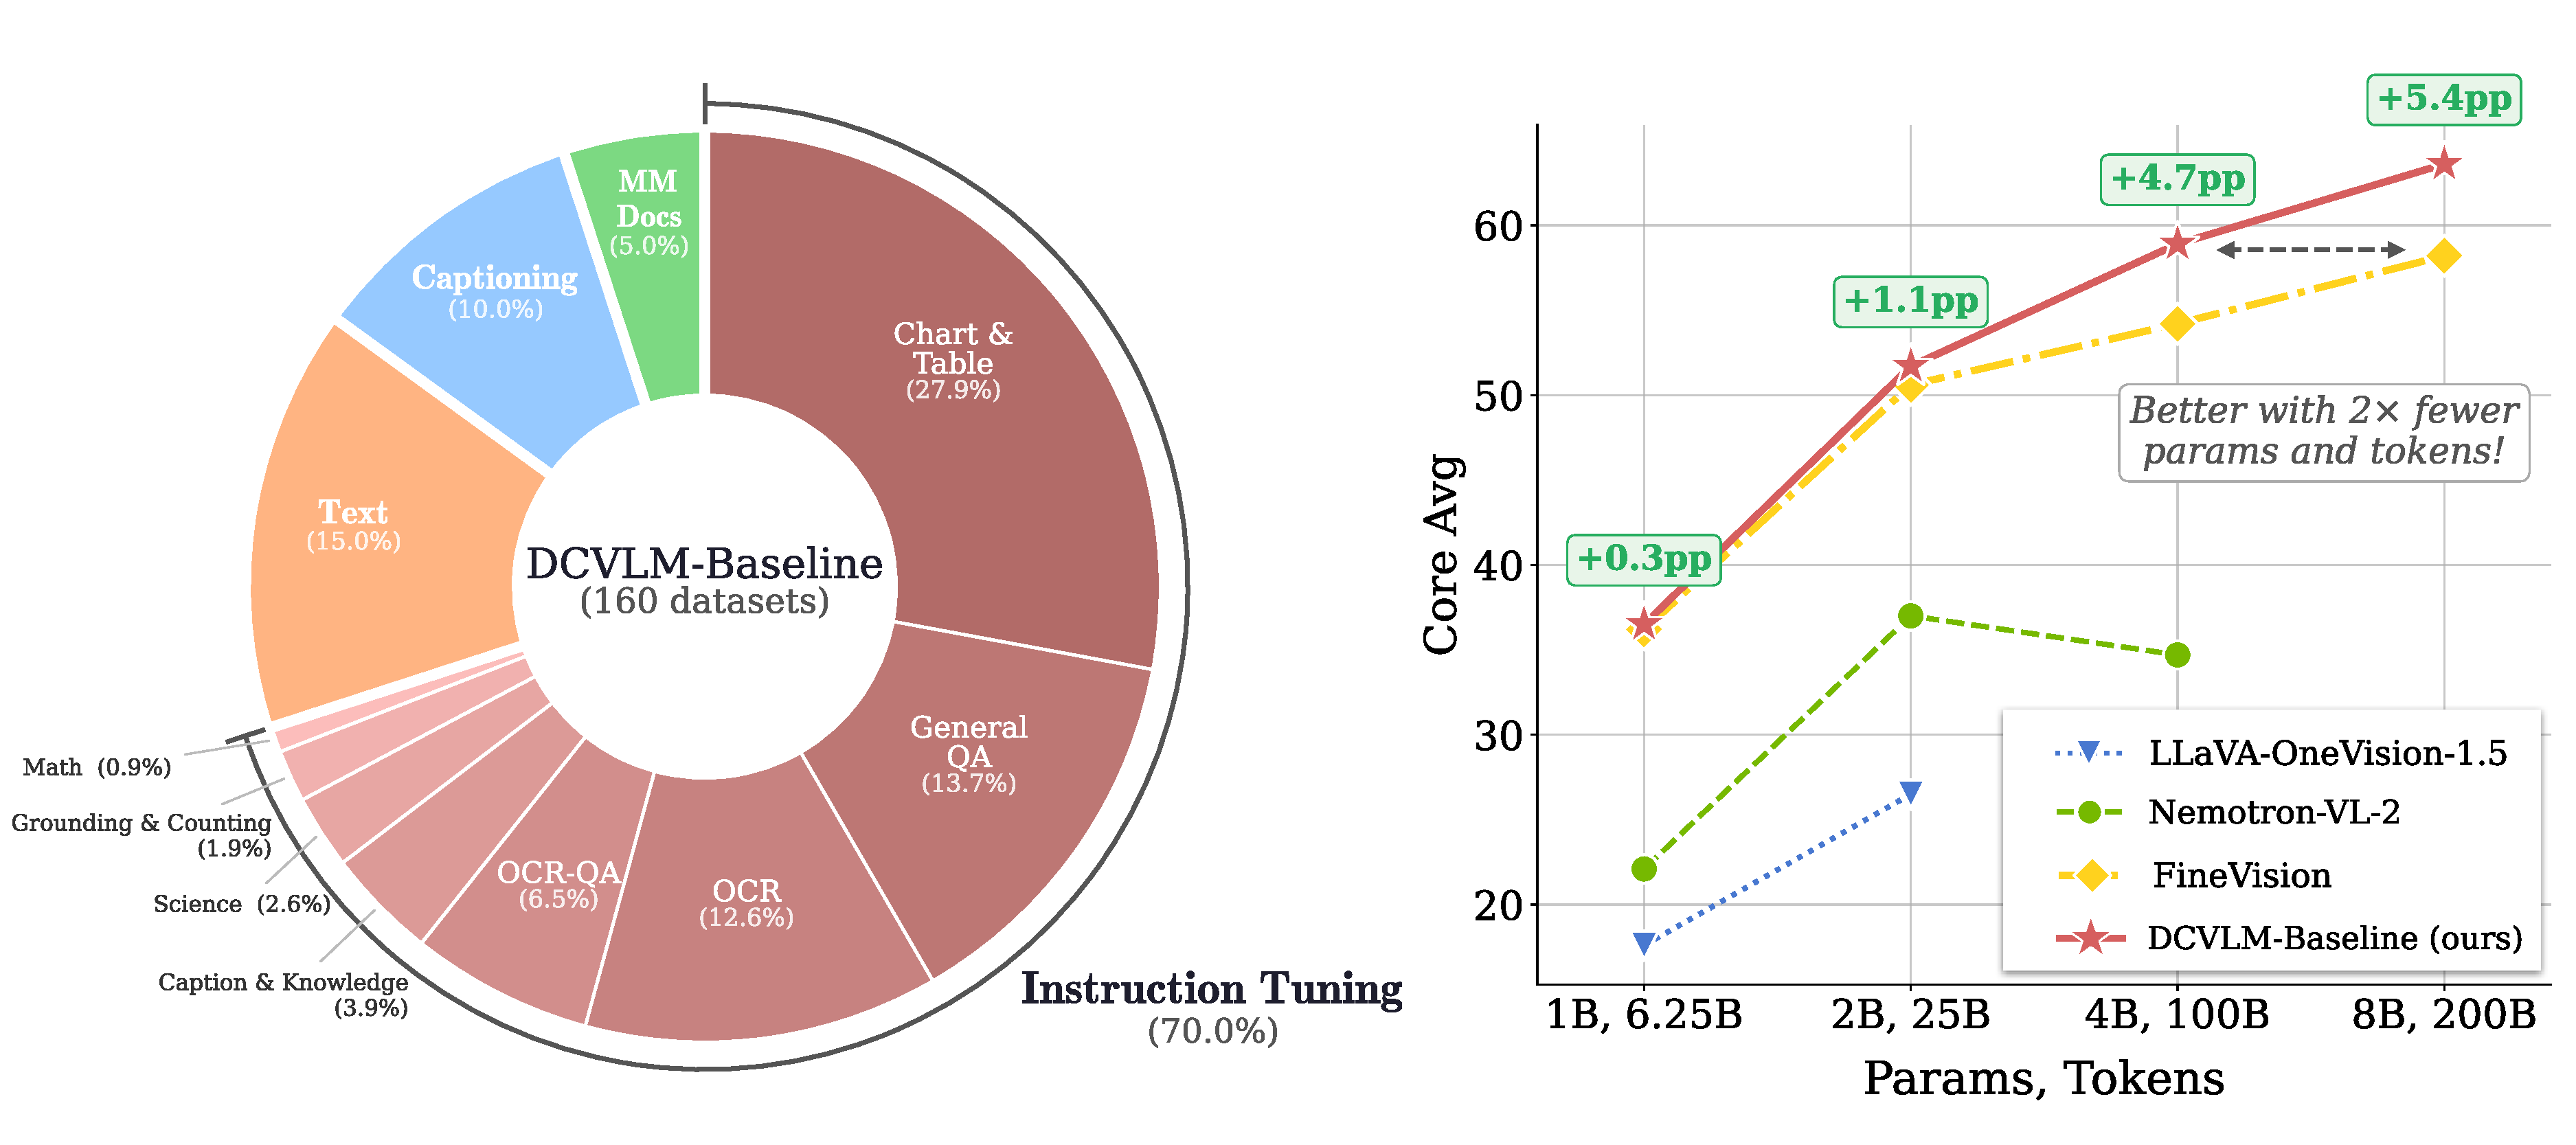
\includegraphics[width=0.95\linewidth]{figures/dcvlm-fig-1.pdf}
\caption{\textbf{\textsc{\dcvlm-Baseline} outperforms open VLM training datasets.} \textsc{\dcvlm-Baseline} \textit{(left)} combines 160 sources as $10$\% image-caption pairs, $5$\% multimodal documents, $15$\% text-only, and $70$\% multimodal instruction-tuning data. On our 33-evaluation Core set \textit{(right)}, it outperforms existing datasets~\cite{deshmukh2025nvidia, an2025llava, wiedmann2025finevision} across all scales. Notably, a 4B model trained on \textsc{\dcvlm-Baseline} for 100B tokens beats an 8B model trained on \textsc{FineVision} for 200B tokens, a ${4}{\times}$ compute reduction.}
\label{fig:hero}
\vspace{-1.5em}
\end{figure*}
}

\newcommand{\figscalinggrid}{%
\begin{figure*}[t]
\centering
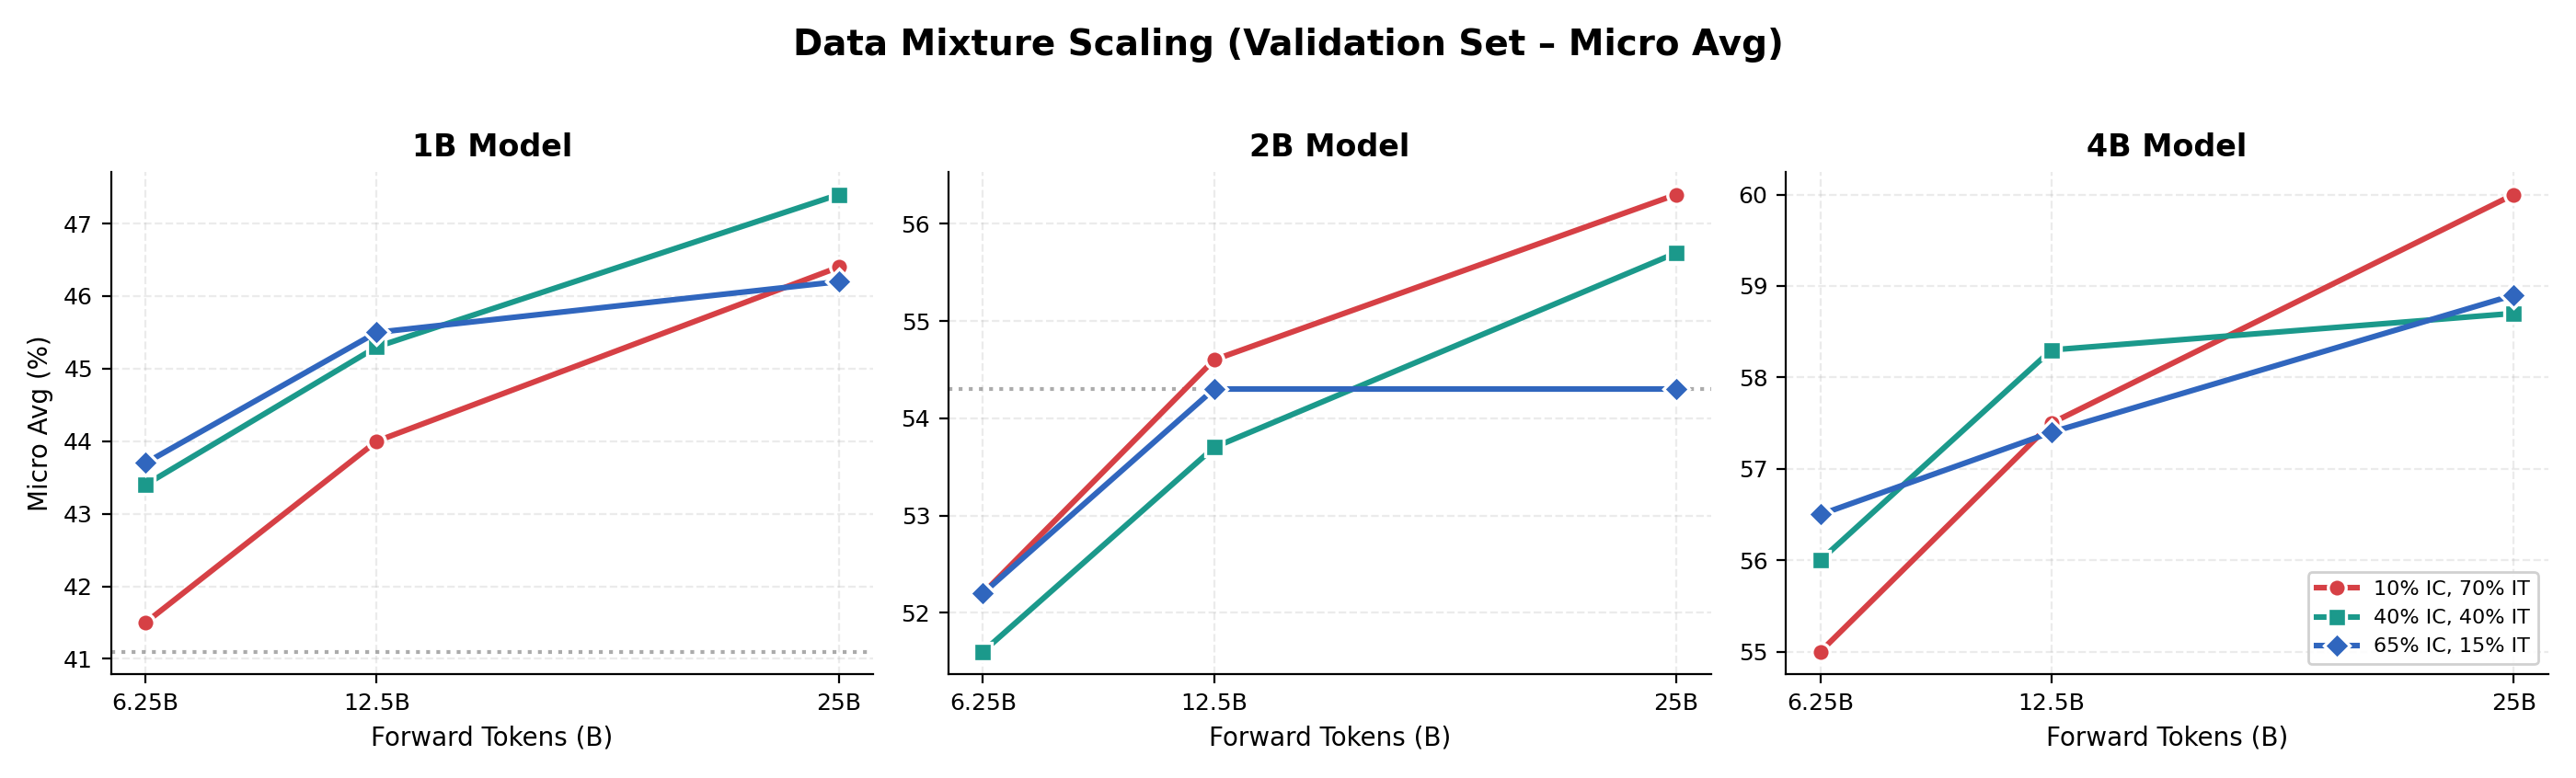
\includegraphics[width=\linewidth]{figures/fig1_scaling_grid_validation.png}
\caption{\textbf{Full scaling grid: 3 data mixtures $\times$ 3 model sizes $\times$ 3 token budgets} (validation set, micro avg). Instruction-heavy mixtures (10c-70i, red) start behind at 1B but overtake at 2B and dominate at 4B. Caption-heavy mixtures (65c-15i, blue) saturate earlier, particularly at 2B where performance plateaus between 12.5B and 25B tokens.}
\label{fig:scaling_grid}
\end{figure*}
}

\newcommand{\figlinesearch}{%
\begin{figure}[t]
\centering
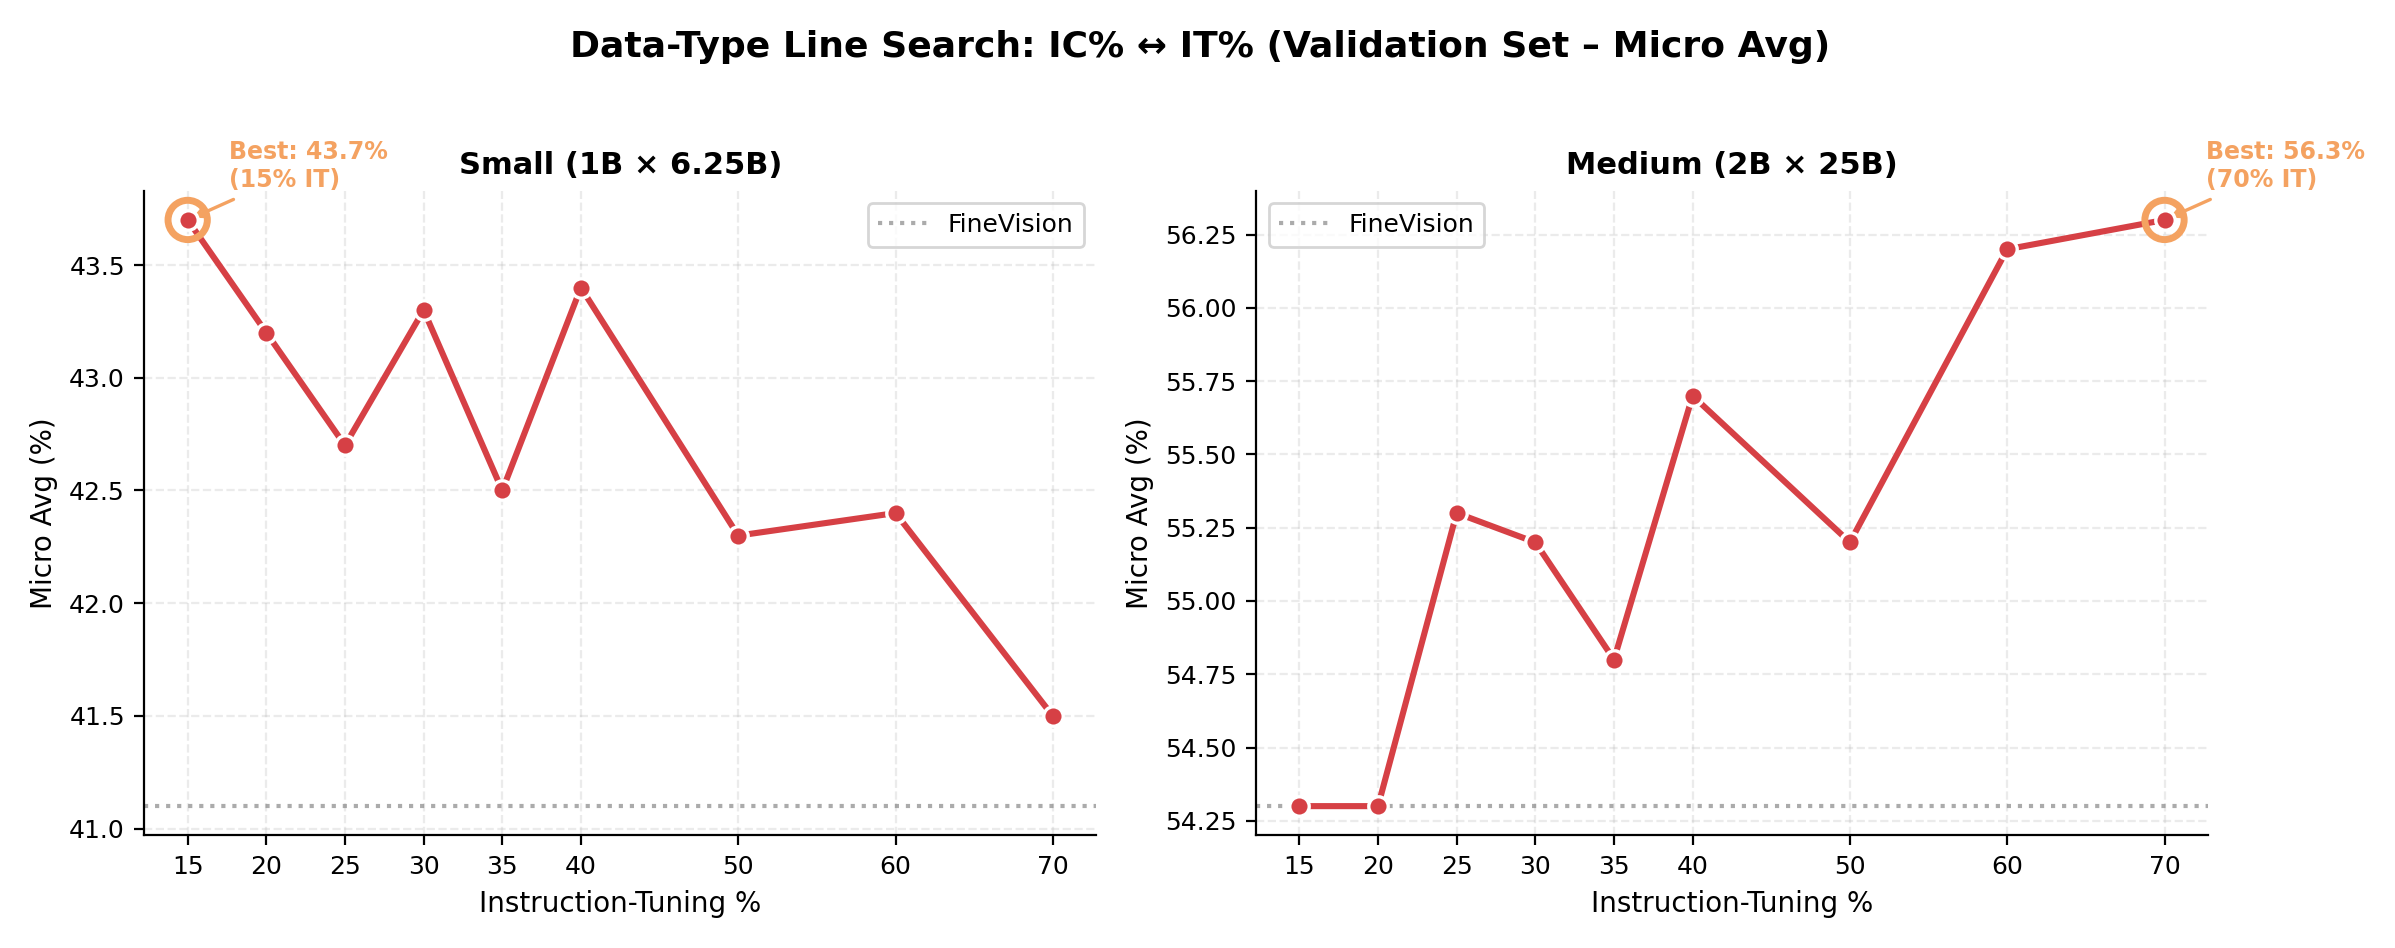
\includegraphics[width=\linewidth]{figures/fig2_line_search_validation.png}
\caption{\textbf{Data-type line search: IC\% $\leftrightarrow$ IT\%.} 9-point sweep at small (1B$\times$6.25B) and medium (2B$\times$25B) scales. At small scale, the 65\%IC baseline is competitive; at medium scale, the optimal shifts to 70\%IT (+2.0\% over baseline). Orange ring highlights the best configuration at each scale.}
\label{fig:line_search}
\end{figure}
}

\newcommand{\figfiltering}{%
\begin{figure*}[t]
\centering
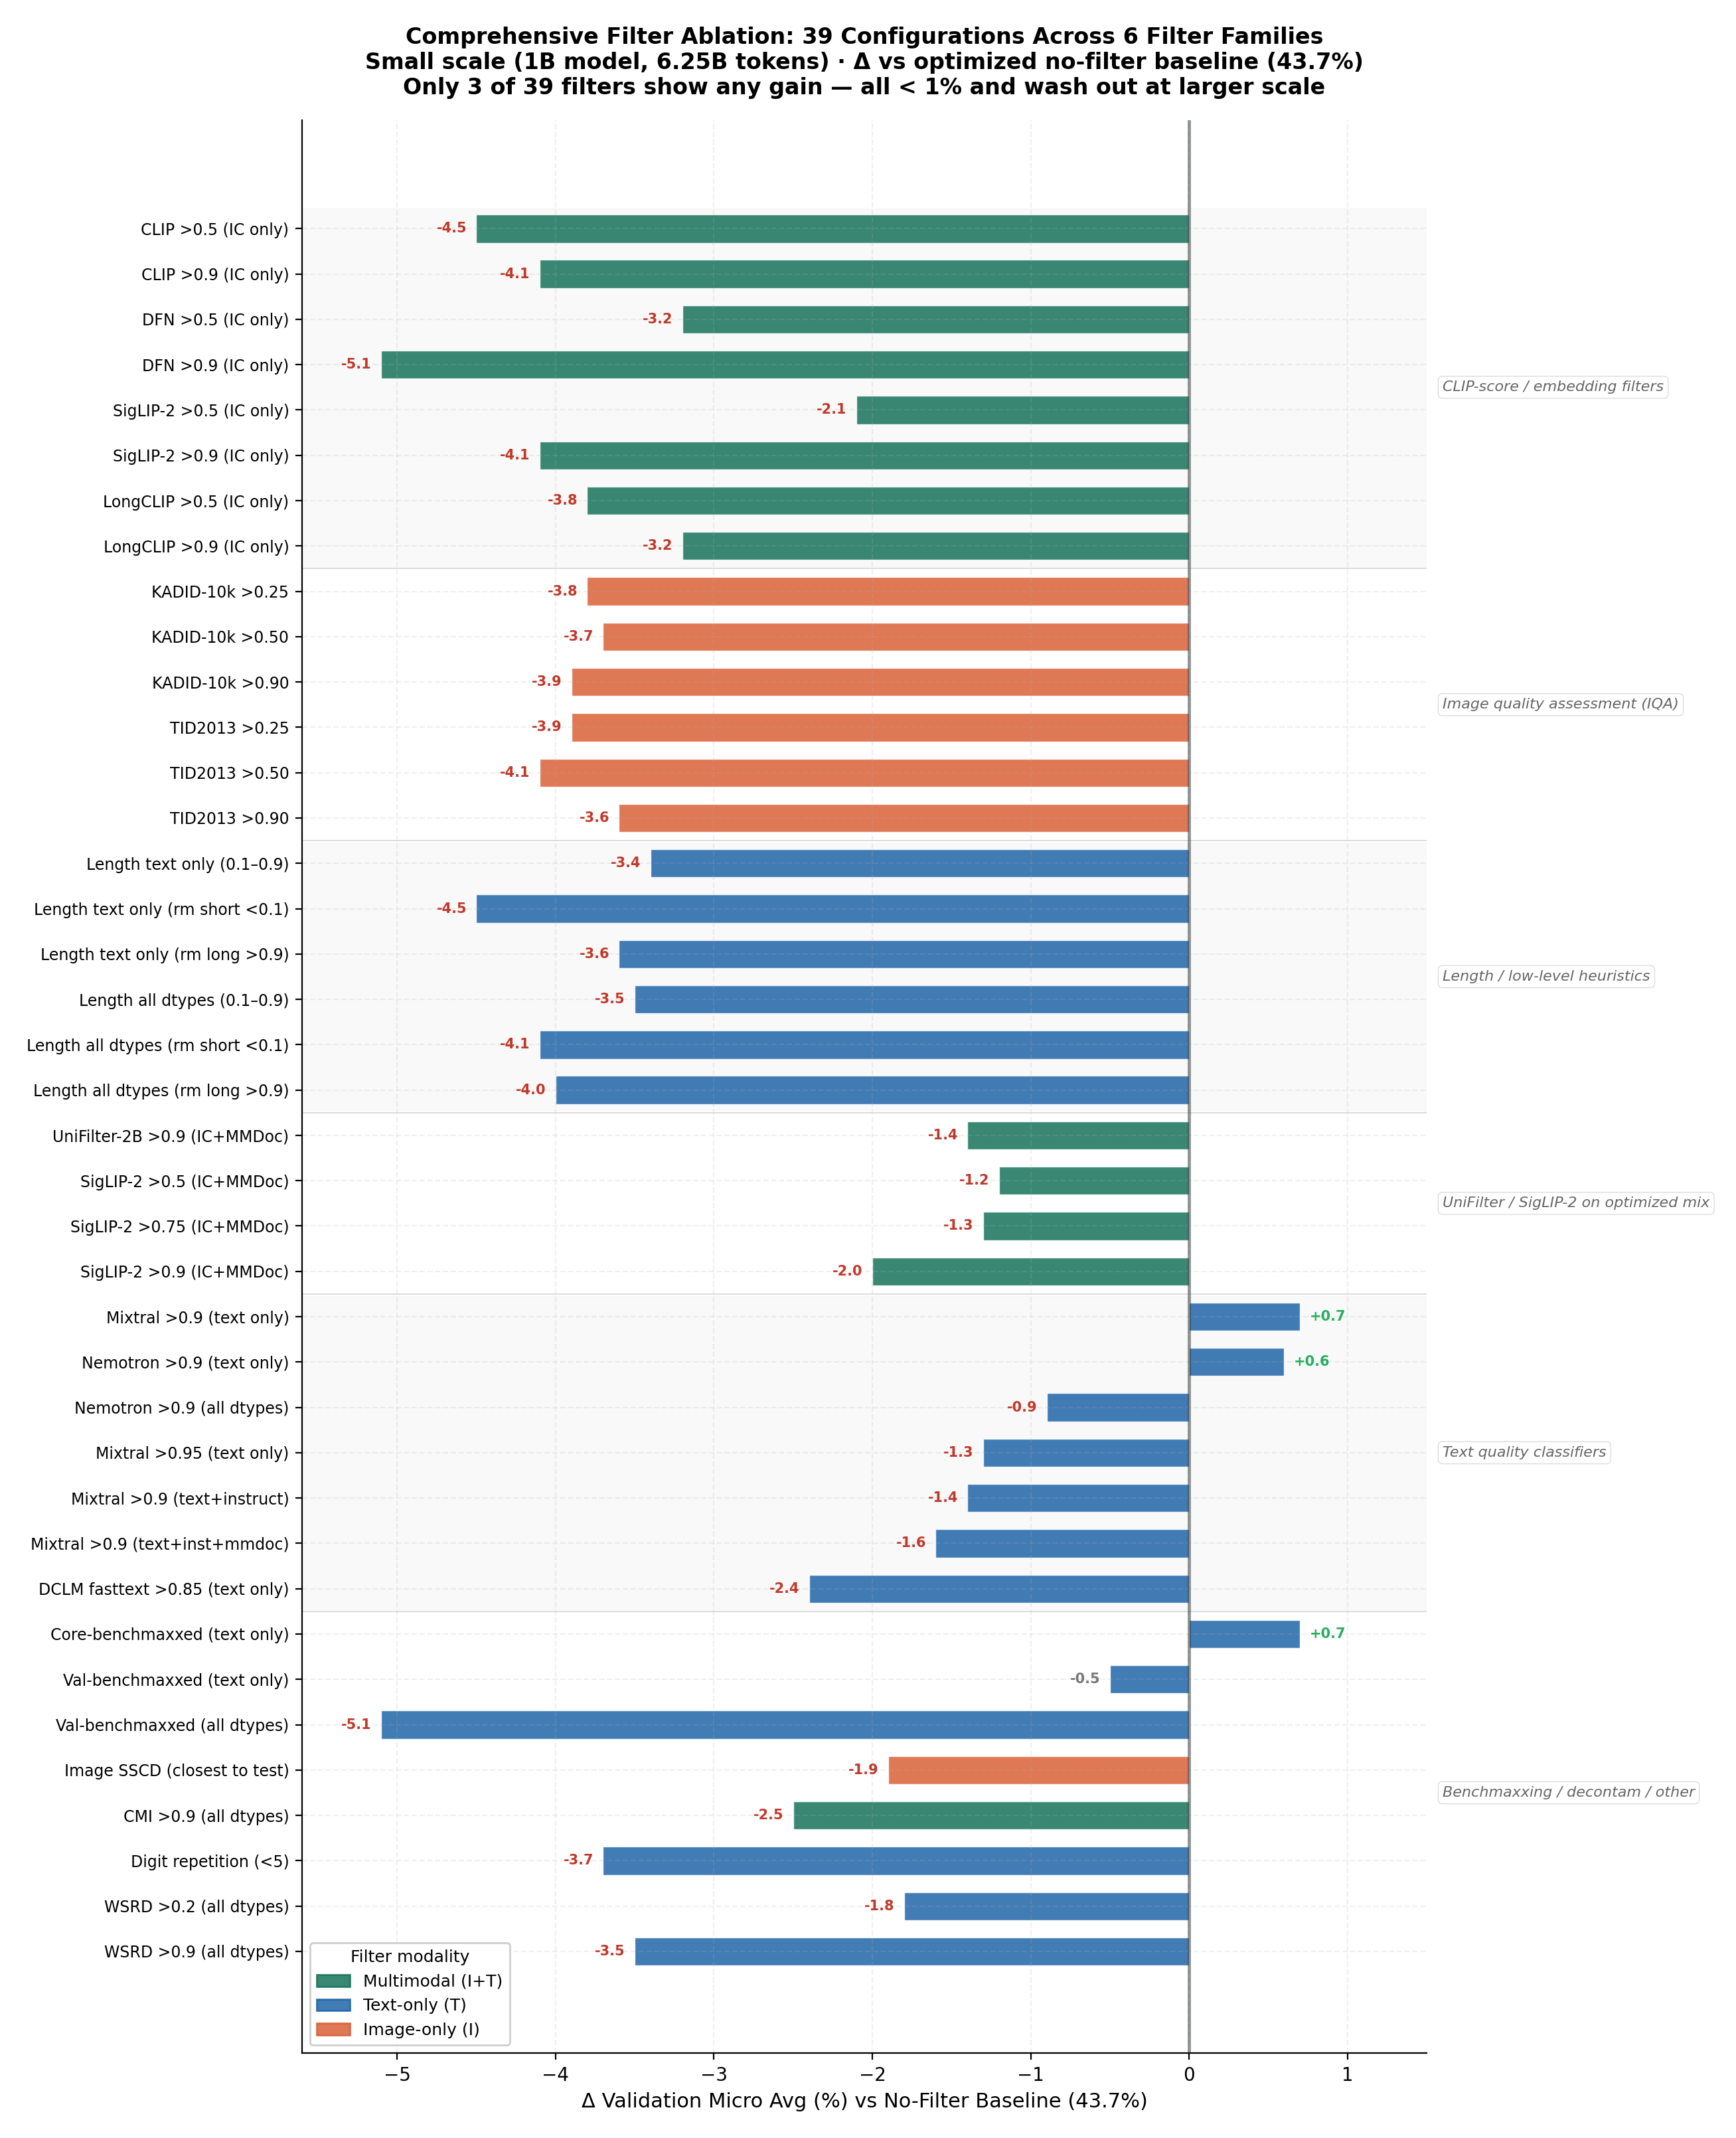
\includegraphics[width=\linewidth]{figures/fig3v2_comprehensive_filtering.png}
\caption{\textbf{Comprehensive filter ablation: 39 configurations across 6 filter families.} Each bar shows $\Delta$ validation micro avg vs.\ the no-filter baseline (43.7\%). Color encodes filter modality: green = multimodal, blue = text-only, orange = image-only. Only 3 of 39 configurations show gains $\geq$+0.5\%, all from text quality classifiers applied exclusively to the text-only data pool.}
\label{fig:filtering}
\end{figure*}
}

\newcommand{\figwashout}{%
\begin{figure}[t]
\centering
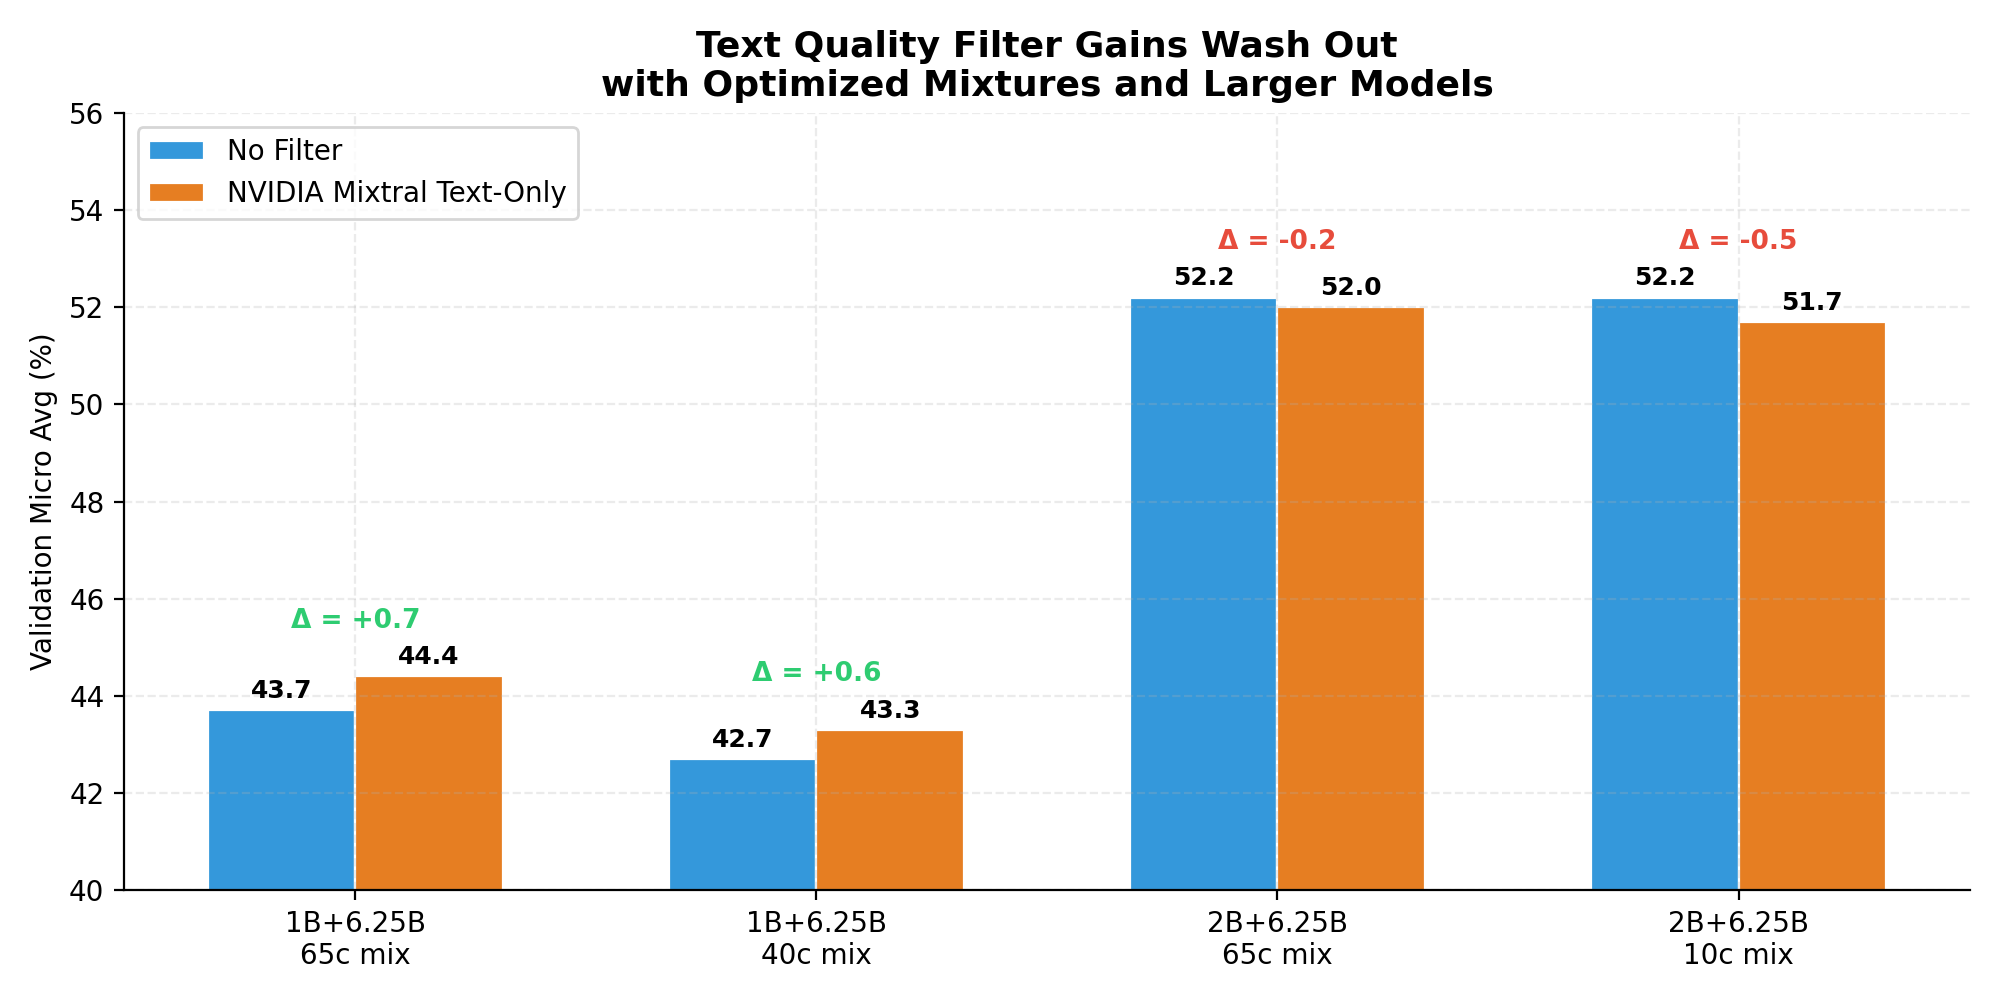
\includegraphics[width=\linewidth]{figures/fig4_filter_washout.png}
\caption{\textbf{Text quality filter gains wash out} with optimized mixtures and larger models. The +0.7\% gain at 1B/65c disappears at 2B/10c ($\Delta = -0.5\%$).}
\label{fig:washout}
\end{figure}
}

\newcommand{\figsampling}{%
\begin{figure}[t]
\centering
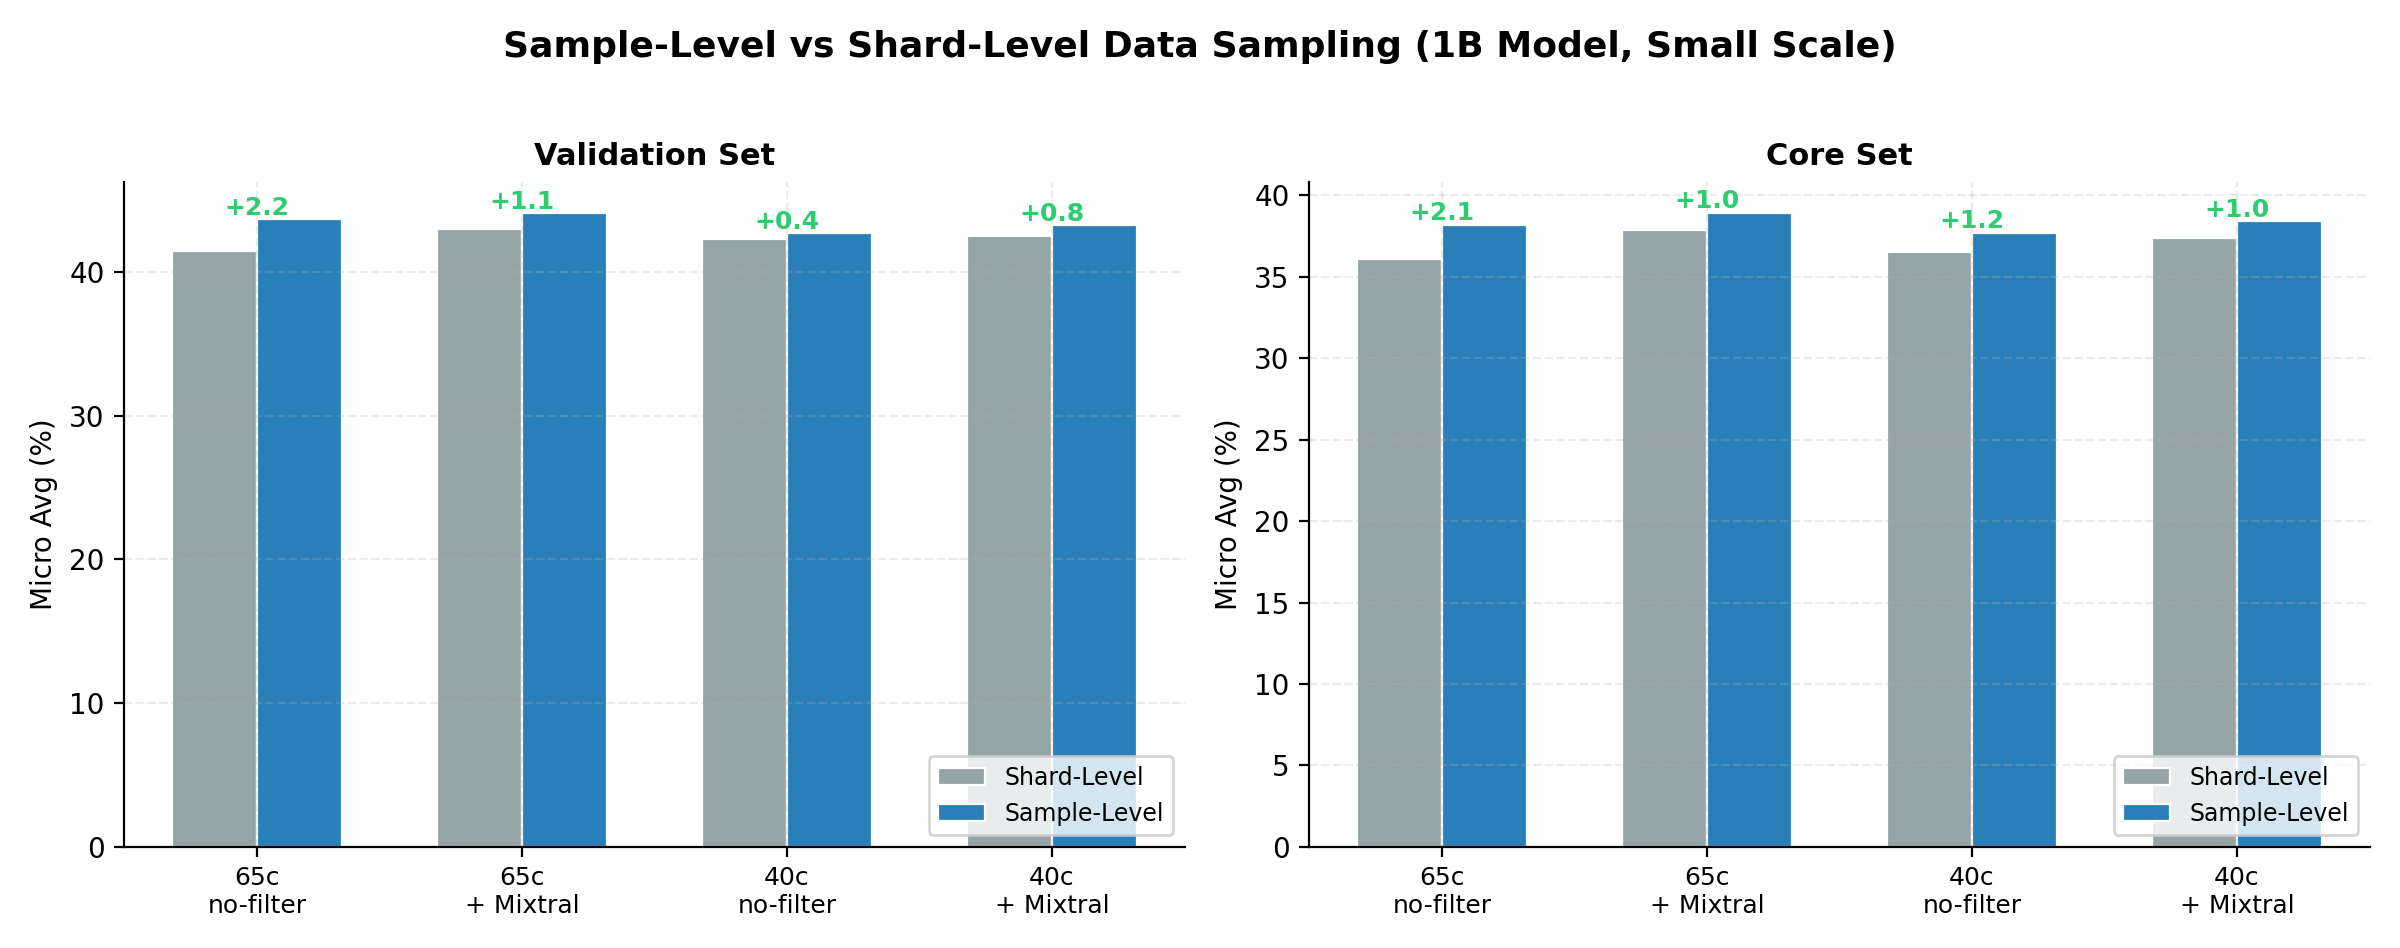
\includegraphics[width=\linewidth]{figures/fig5_sampling_strategy.png}
\caption{\textbf{Sample-level vs.\ shard-level data sampling} (1B model, small scale). Sample-level sampling provides a consistent +1--2\% improvement across all configurations, rivaling the best filtering results.}
\label{fig:sampling}
\end{figure}
}

\newcommand{\figtemperature}{%
\begin{figure}[t]
\centering
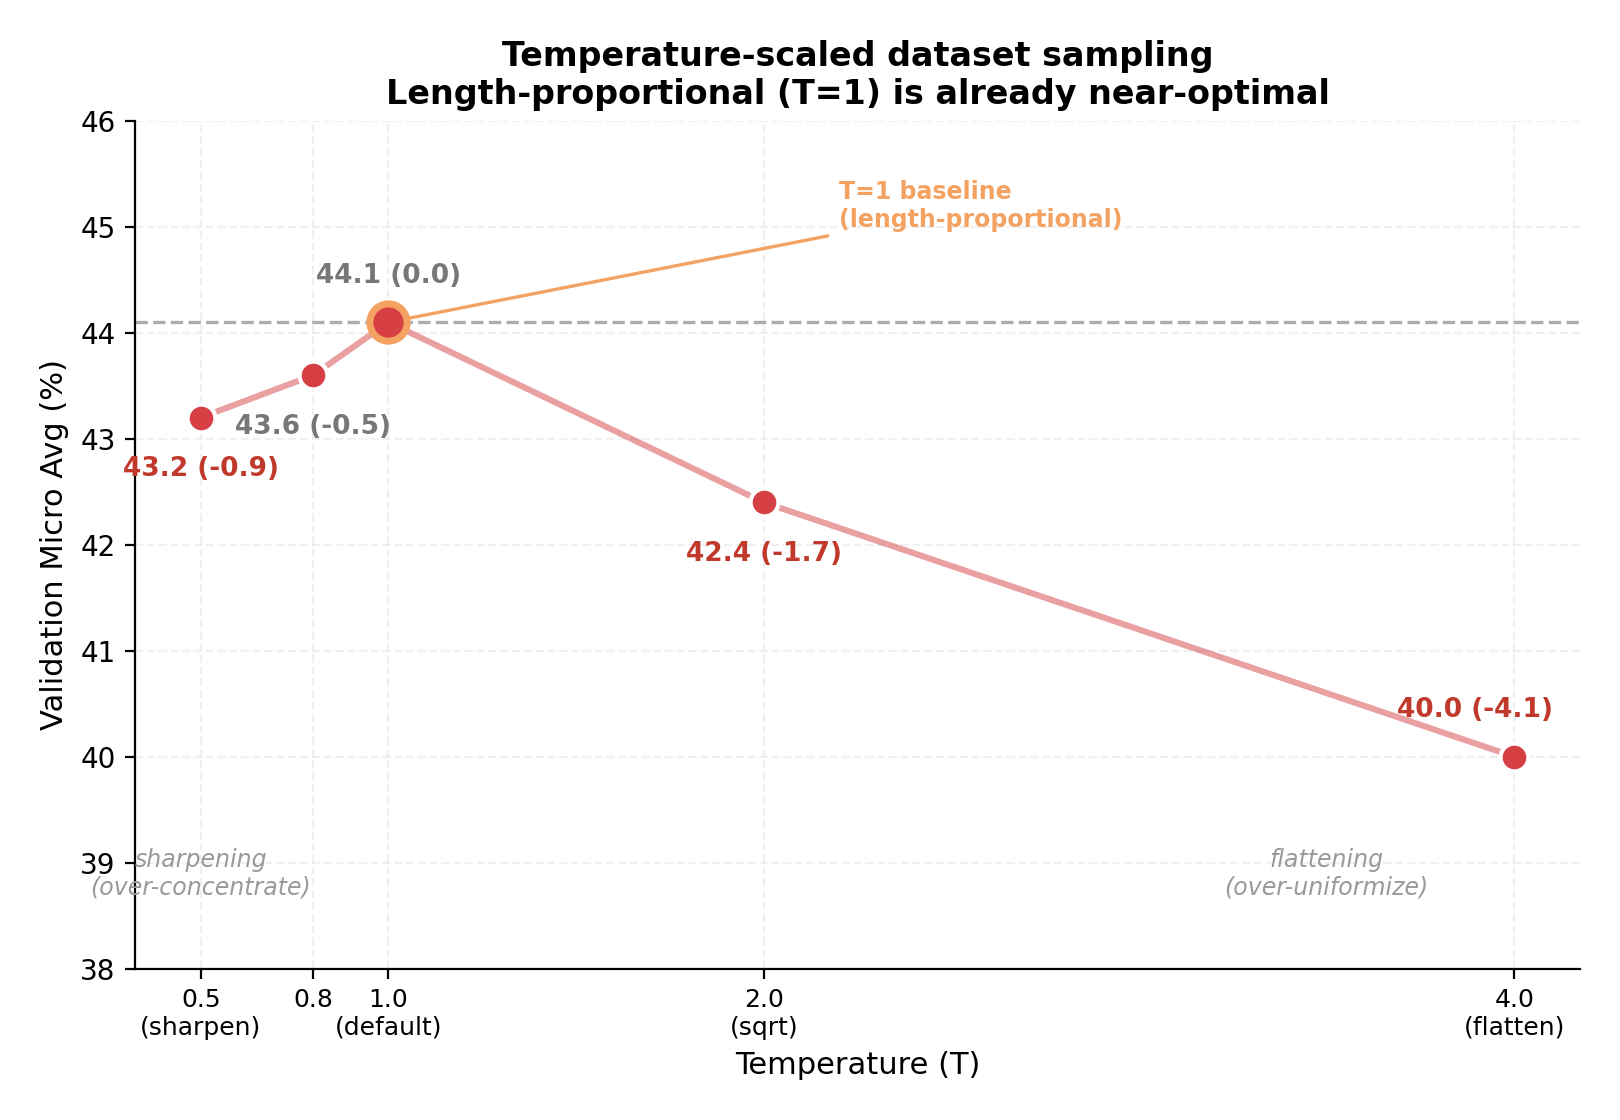
\includegraphics[width=\linewidth]{figures/fig10_temperature_sampling.png}
\caption{\textbf{Temperature-scaled dataset sampling.} $T=1$ (length-proportional, the default) is near-optimal. Both flattening ($T \geq 2$) and sharpening ($T < 1$) degrade performance, with $T=4$ dropping 4.1\% below baseline.}
\label{fig:temperature}
\end{figure}
}

\newcommand{\figlargescale}{%
\begin{figure}[t]
\centering
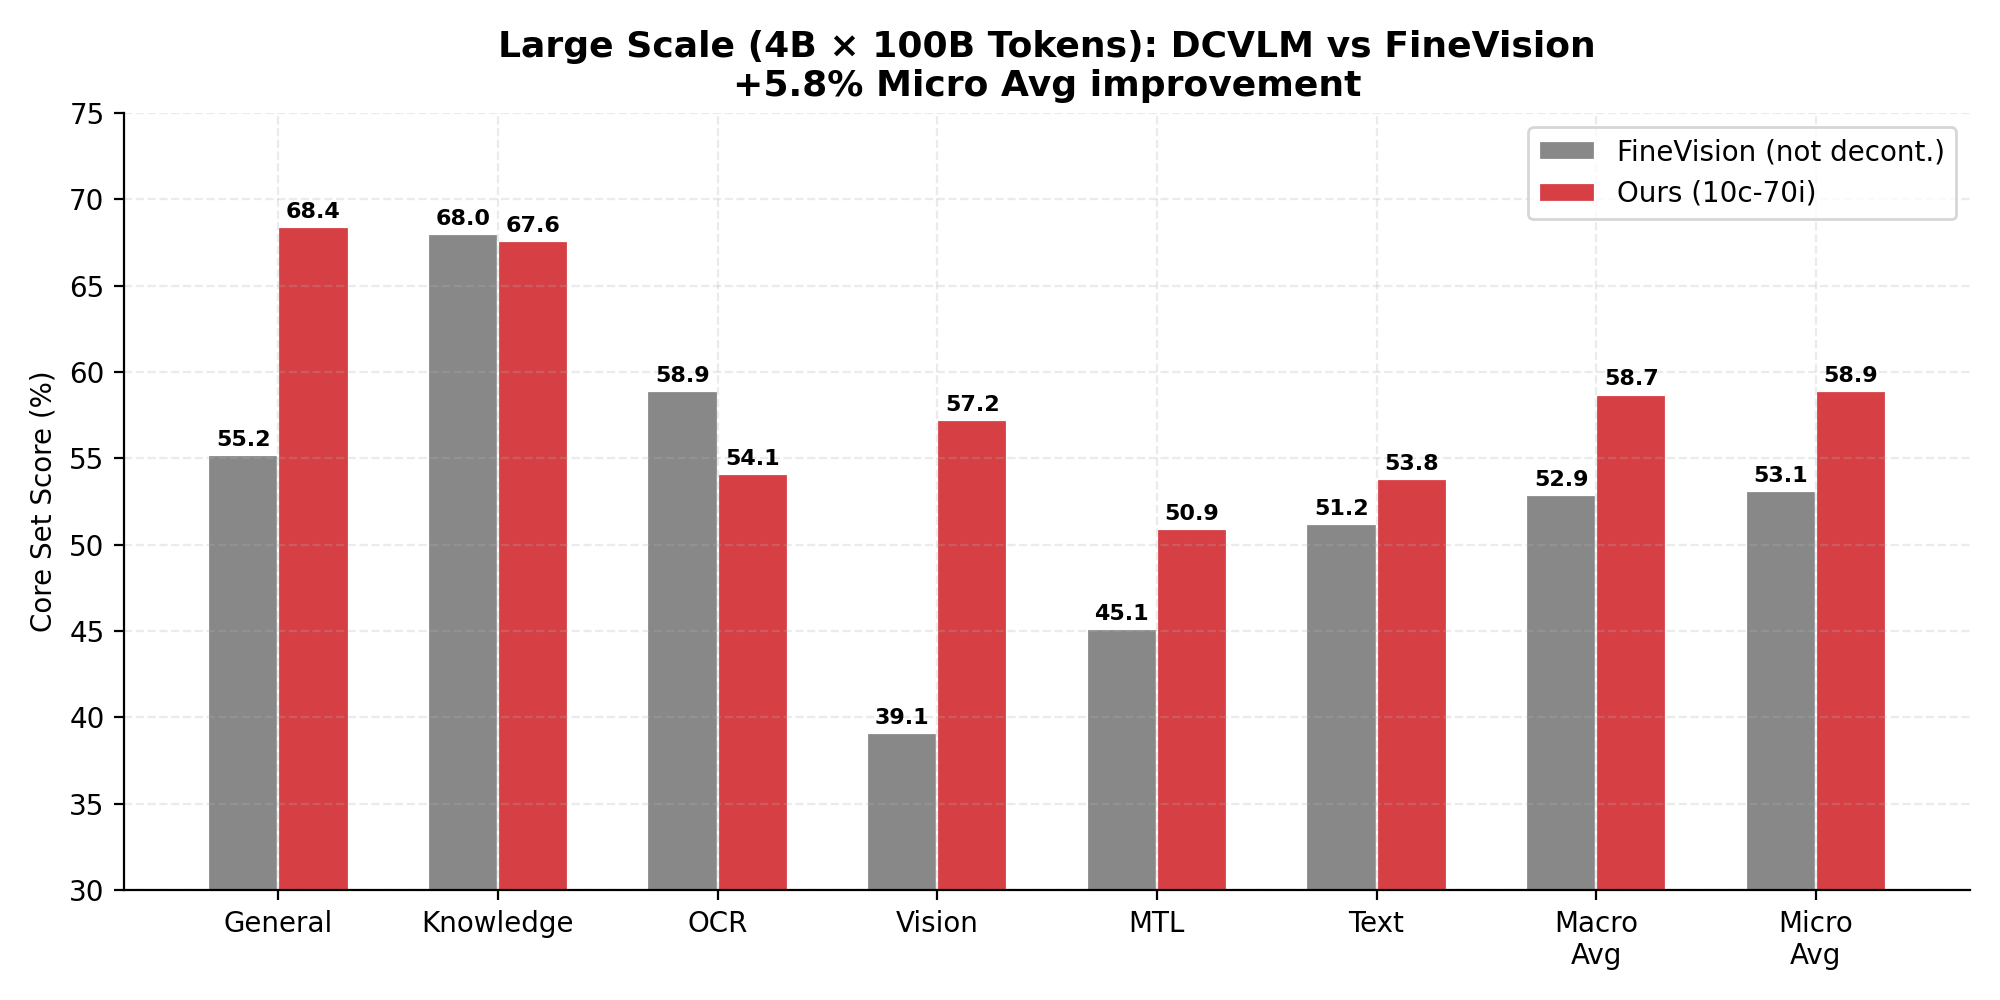
\includegraphics[width=\linewidth]{figures/fig6_large_scale.png}
\caption{\textbf{Large scale (4B$\times$100B): per-category core-set comparison.} \dcvlm outperforms \fv on 5 of 6 categories (+13.2\% General, +18.1\% Vision), trailing only on OCR ($-$4.8\%).}
\label{fig:large_scale}
\end{figure}
}

\newcommand{\figfvcontamination}{%
\begin{figure*}[t]
\centering
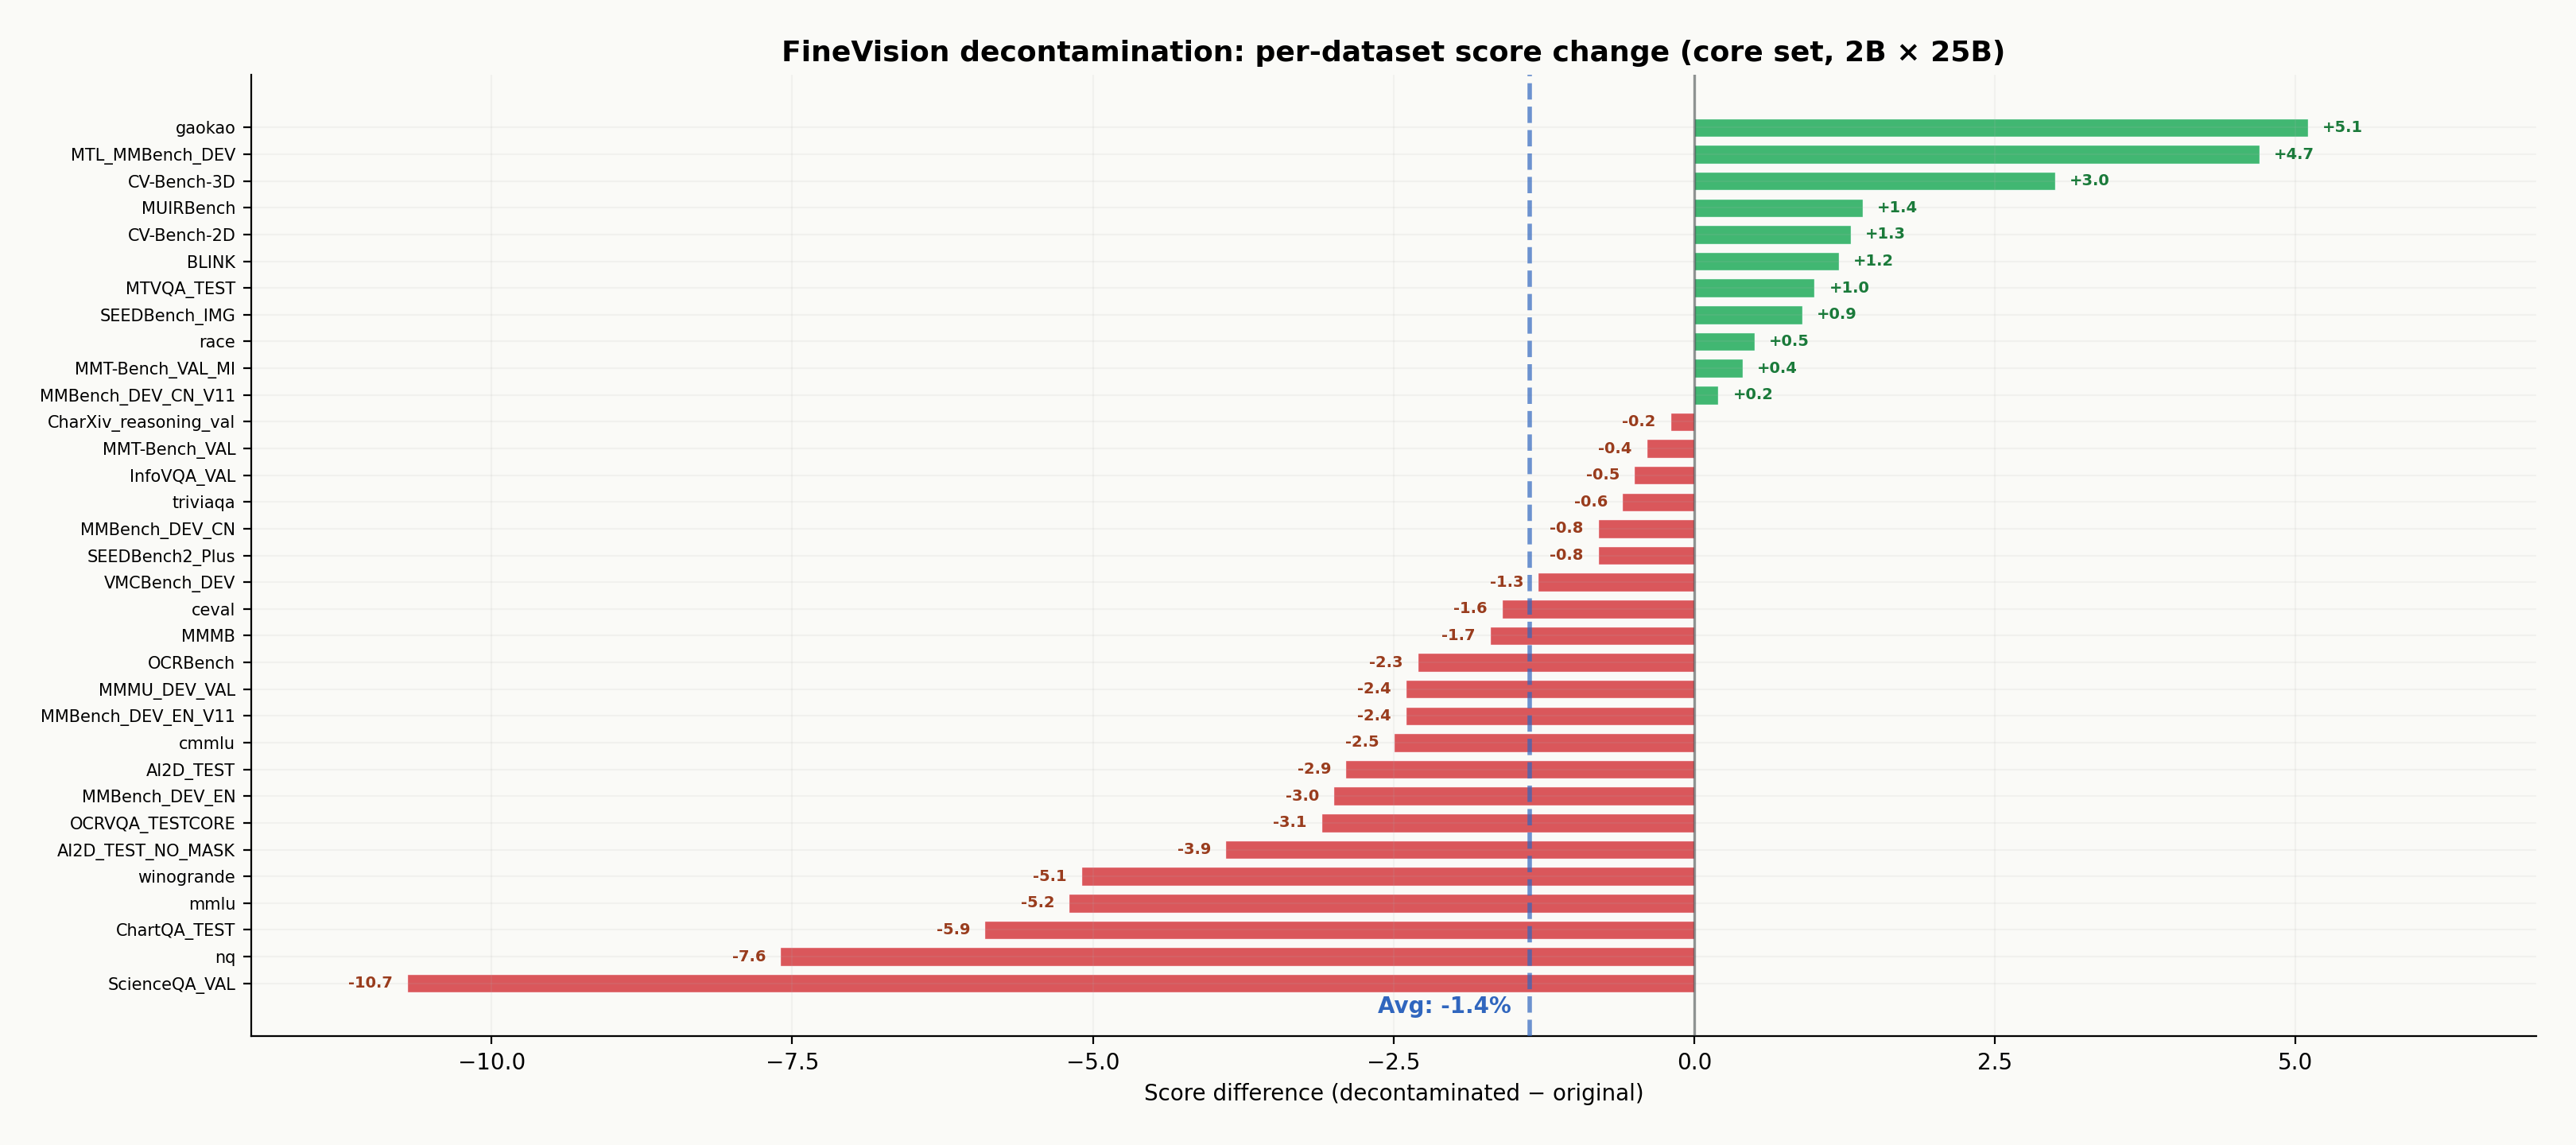
\includegraphics[width=\linewidth]{figures/fig_fv_decontamination_perdataset.png}
\caption{\textbf{FineVision decontamination: per-dataset score change} (core set, 2B$\times$25B). Blue dashed line shows the average drop ($-$1.4\%). The largest drops are on ScienceQA ($-$10.7\%), nq ($-$7.6\%), and ChartQA ($-$5.9\%)---precisely the categories where \fv appeared strongest.}
\label{fig:fv_contamination}
\end{figure*}
}

\newcommand{\figocr}{%
\begin{figure}[t]
\centering
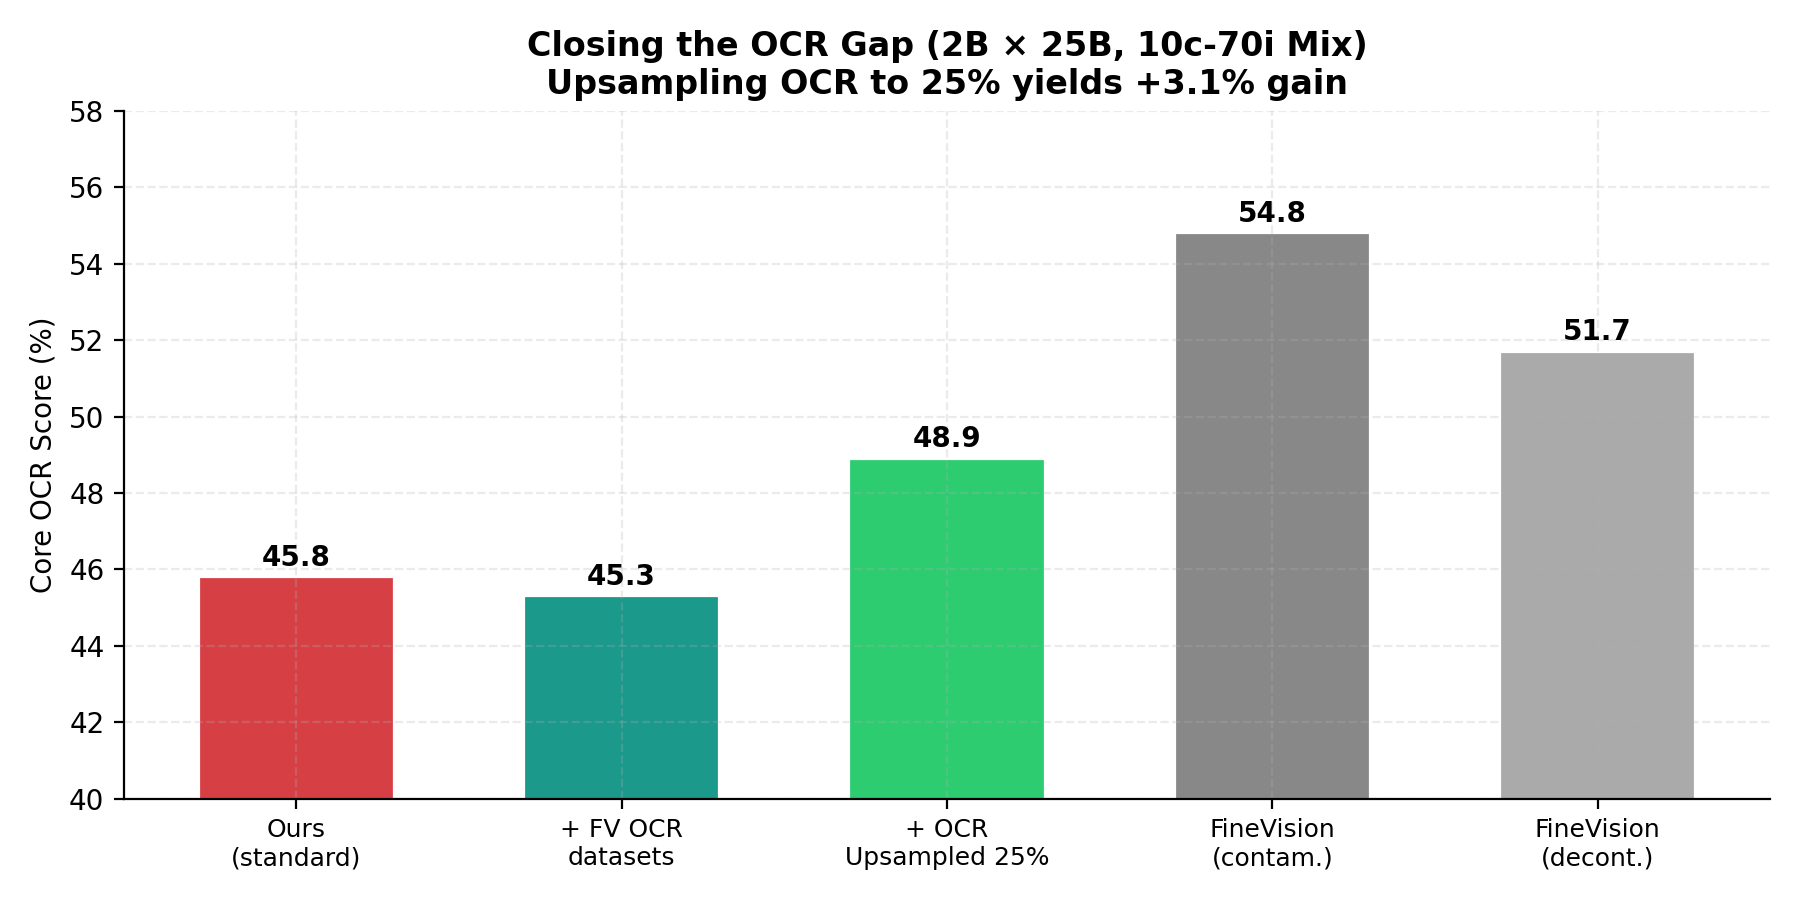
\includegraphics[width=0.9\linewidth]{figures/fig8_ocr_upsampling.png}
\caption{\textbf{Closing the OCR gap} (2B$\times$25B, 10c-70i mix). Upsampling OCR data from 17\% to 25\% yields +3.1\% on the core OCR category, closing roughly half the remaining gap with decontaminated \fv.}
\label{fig:ocr}
\end{figure}
}

\newcommand{\figonlinefiltering}{%
\begin{figure*}[t]
\centering
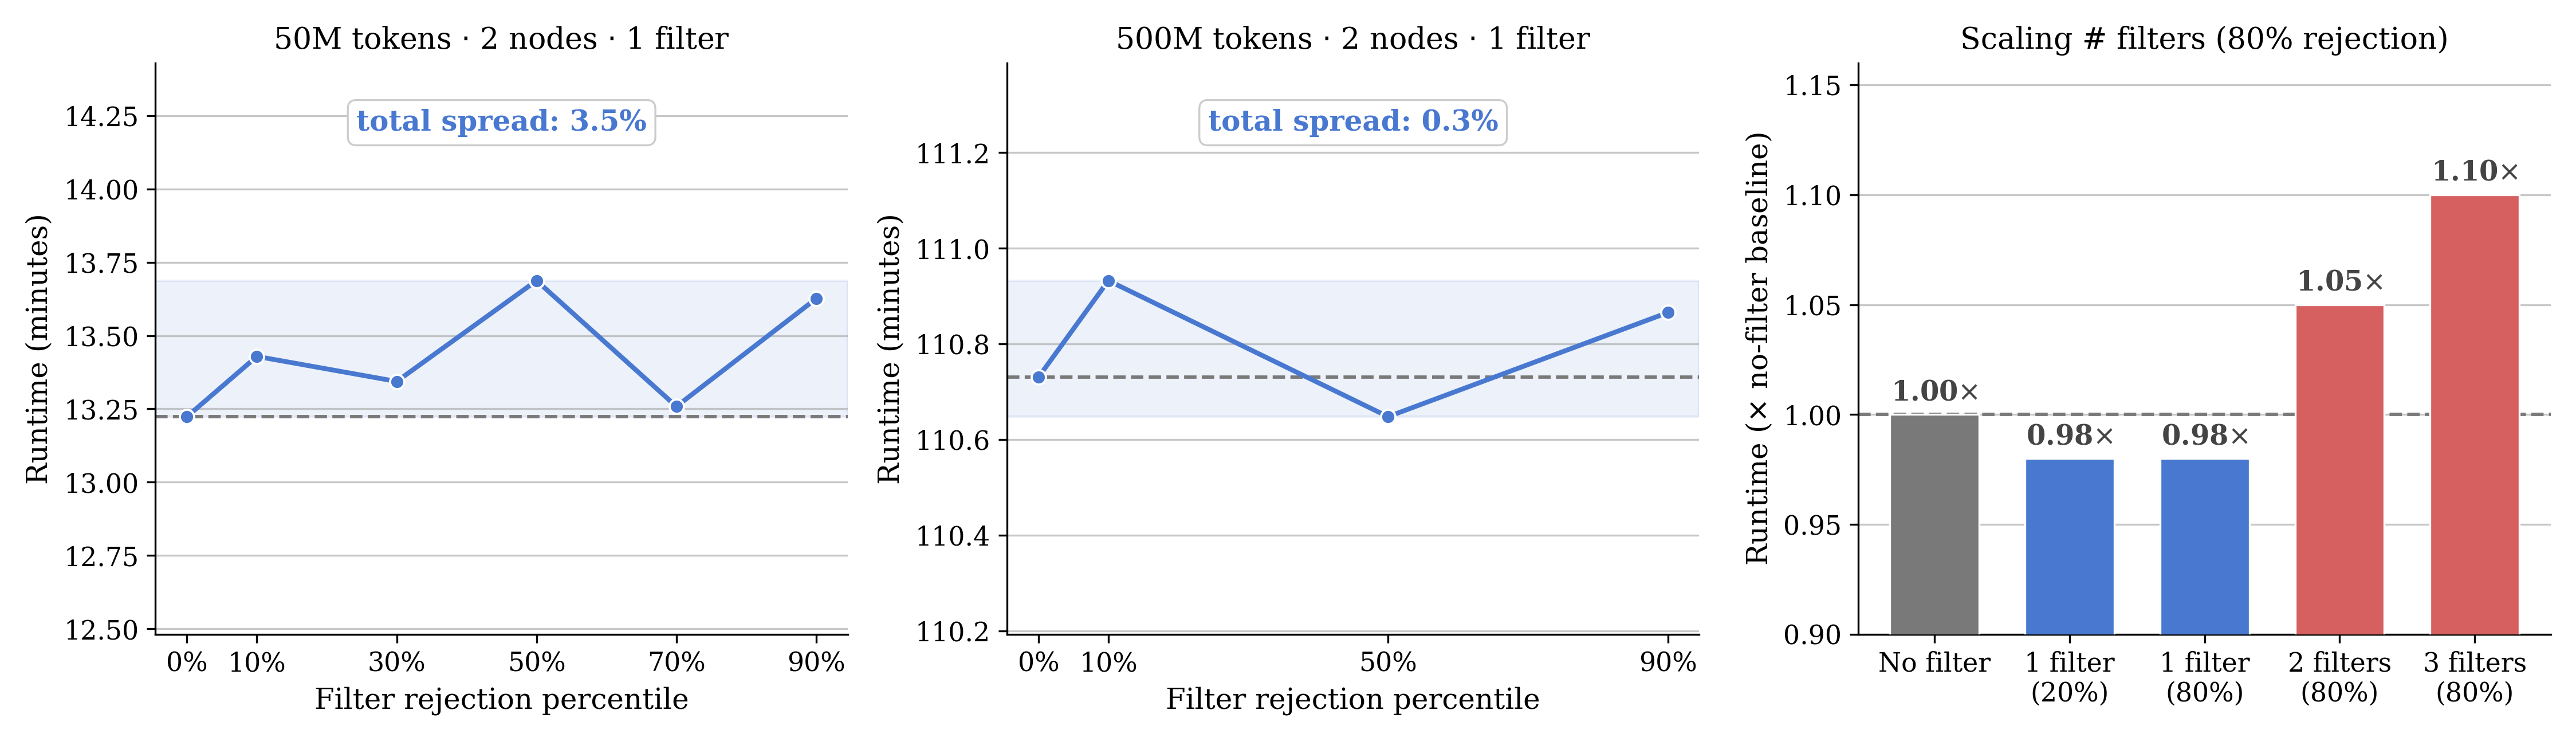
\includegraphics[width=\linewidth]{figures/fig_online_filtering_overhead.png}
\caption{\textbf{Online filtering adds negligible overhead.} \emph{Left/Center:} Varying rejection percentile from 0\% to 90\% with 1 filter yields 3.5\% total spread at 50M tokens and only 0.3\% at 500M tokens. \emph{Right:} Scaling to 3 filters at 80\% rejection each costs only 1.10$\times$ baseline runtime.}
\label{fig:online_filtering}
\end{figure*}
}

\newcommand{\figrecaptioning}{%
\begin{figure}[t]
\centering
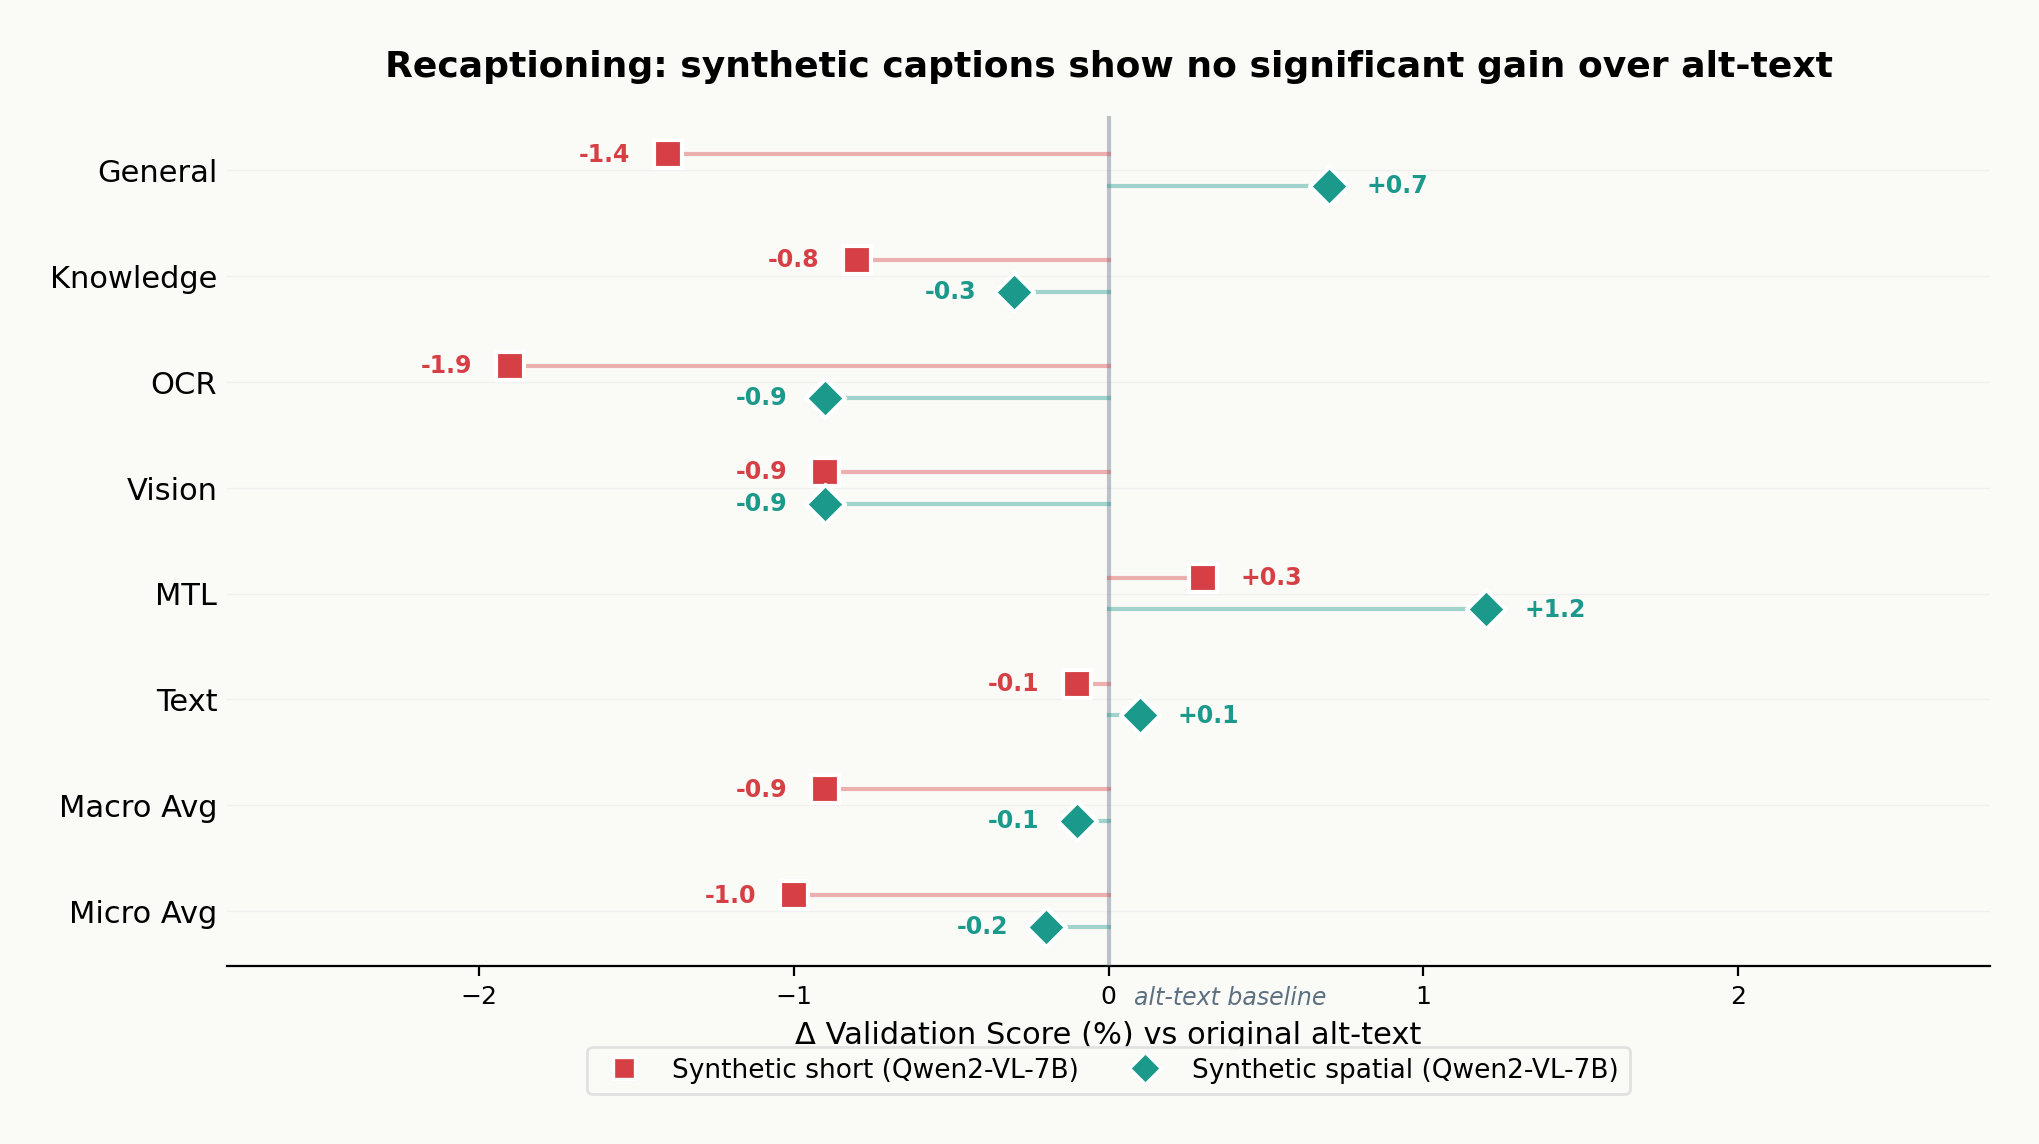
\includegraphics[width=\linewidth]{figures/fig9_recaptioning.png}
\caption{\textbf{Recaptioning: synthetic captions $\approx$ alt-text.} Detrended lollipop plot showing deltas from the alt-text baseline. No caption type significantly outperforms original alt-text at the VLM pretraining stage.}
\label{fig:recaptioning}
\end{figure}
}

\newcommand{\figisocompute}{%
\begin{figure}[t]
\centering
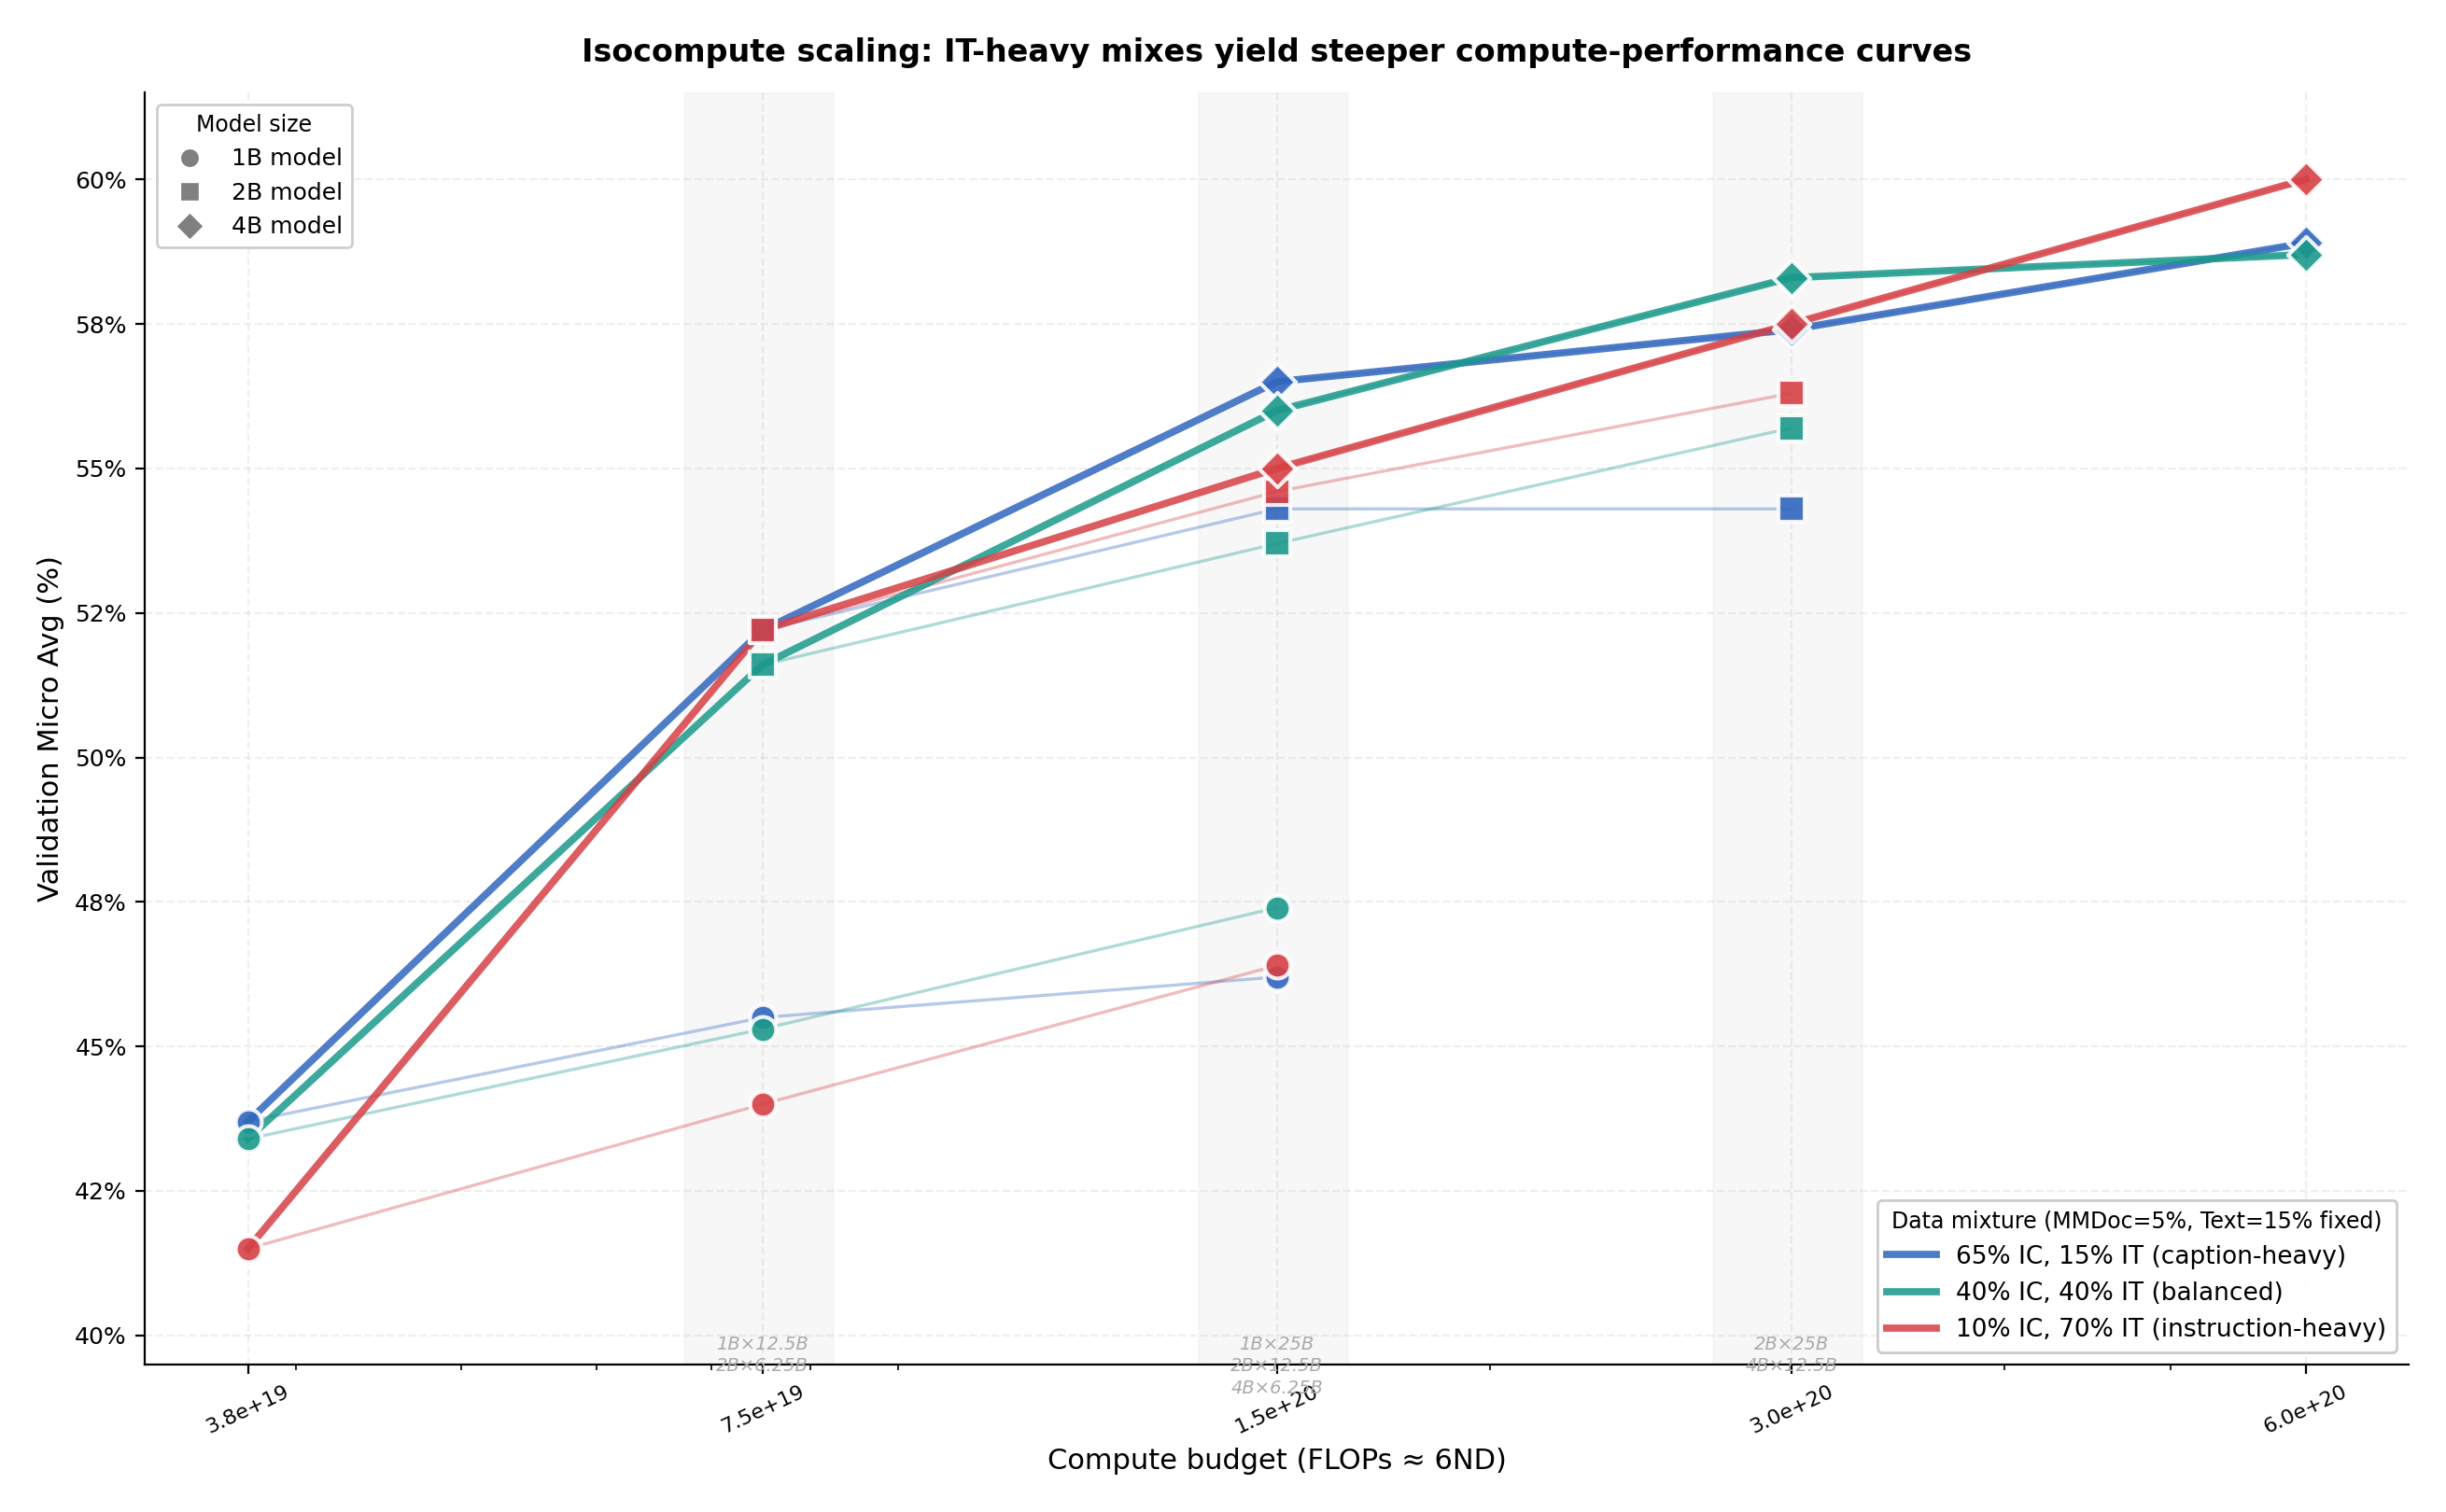
\includegraphics[width=\linewidth]{figures/fig_isocompute.png}
\caption{\textbf{Isocompute scaling curves.} Validation micro avg as a function of training FLOPs (log scale) for each data mixture$\times$model combination. IT-heavy mixtures show steeper slopes, indicating more efficient use of additional compute.}
\label{fig:isocompute}
\end{figure}
}

\newcommand{\figmixinteraction}{%
\begin{figure}[t]
\centering
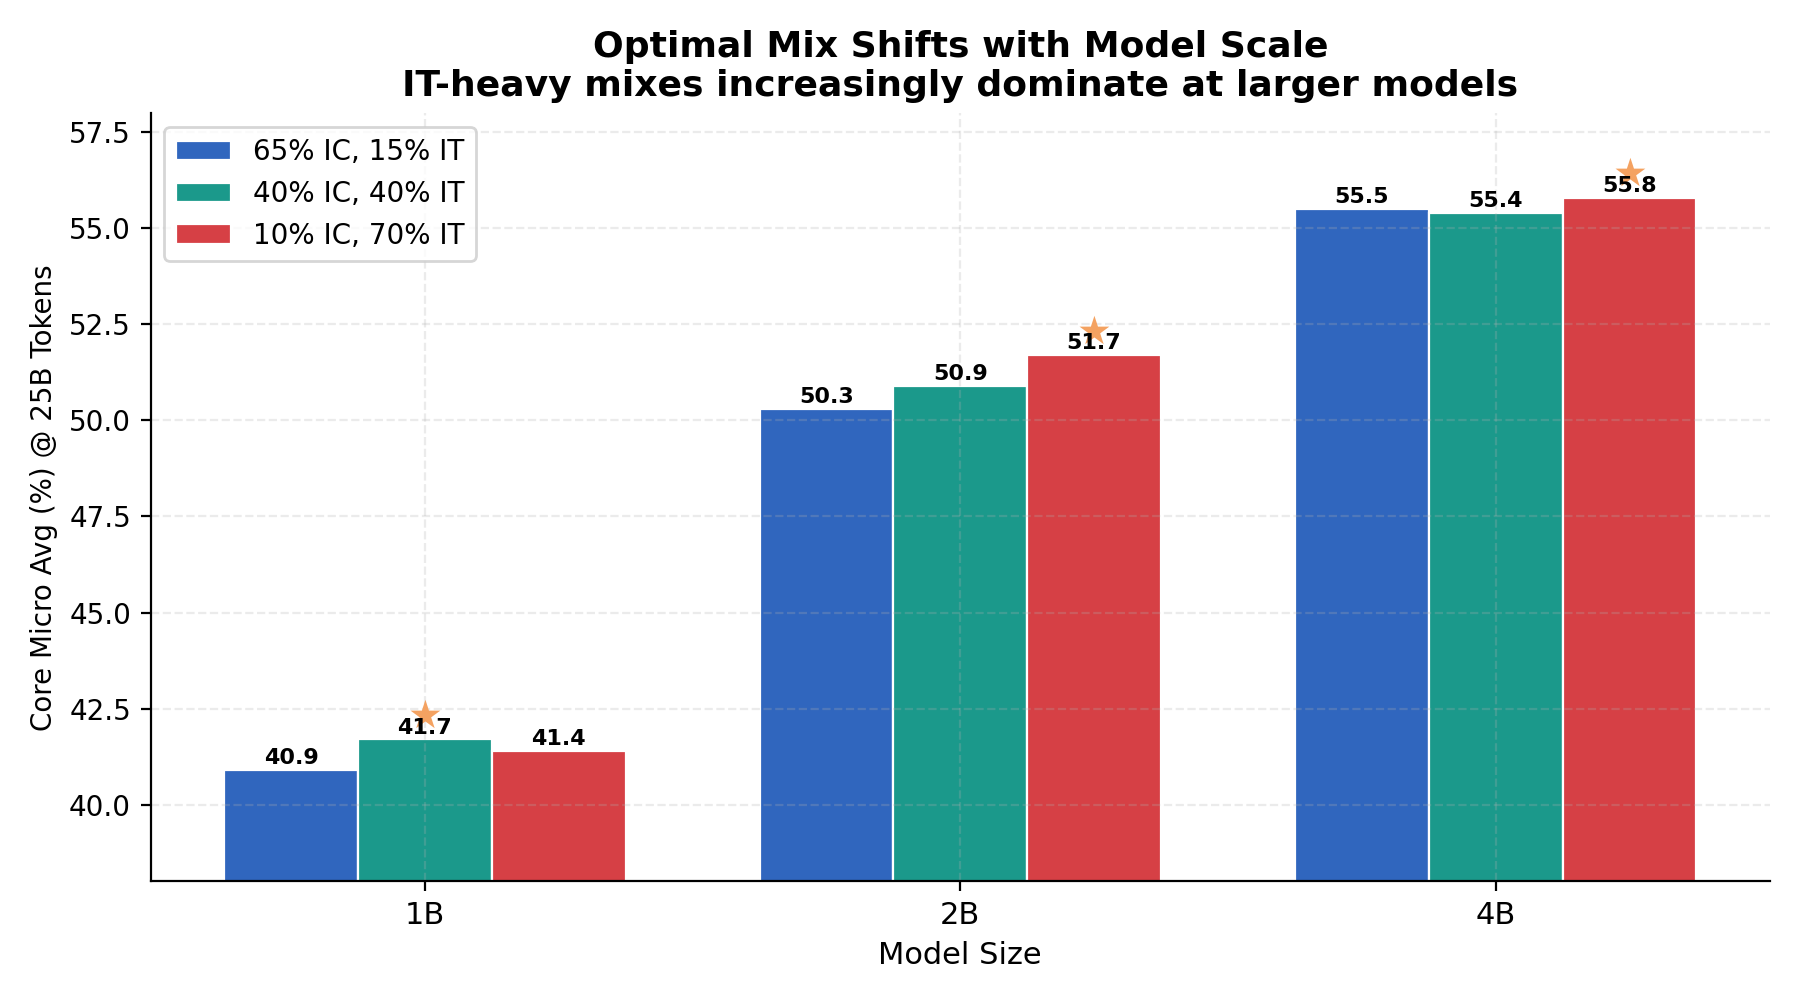
\includegraphics[width=0.9\linewidth]{figures/fig14_model_mix_interaction.png}
\caption{\textbf{Optimal mix shifts with model scale} (core set, 25B tokens). At 1B, balanced (40c) is best; at 2B and 4B, instruction-heavy (10c-70i) dominates. Stars mark the best mix per model size.}
\label{fig:mix_interaction}
\end{figure}
}

\newcommand{\figcategorybreakdown}{%
\begin{figure*}[t]
\centering
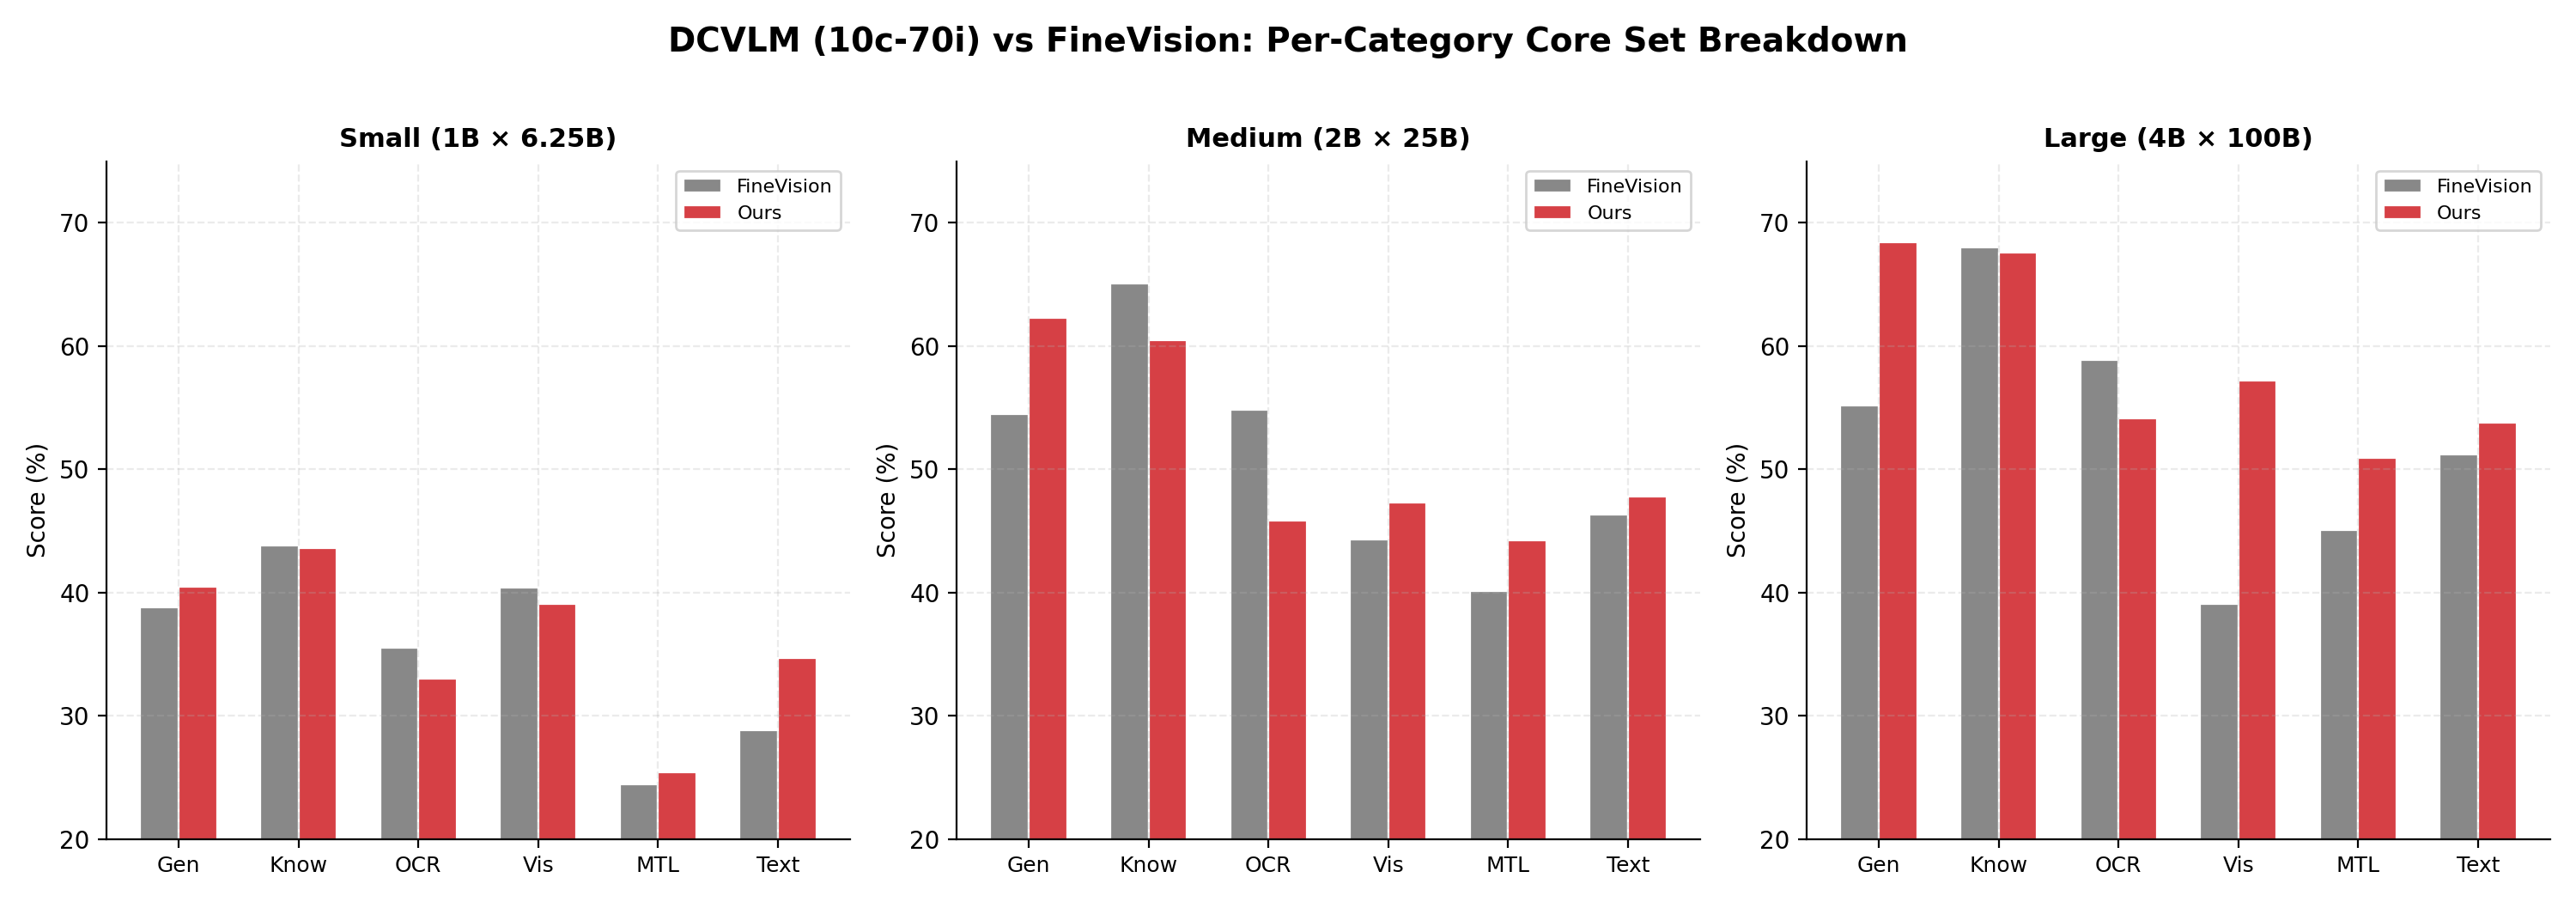
\includegraphics[width=\linewidth]{figures/fig12_category_breakdown_across_scales.png}
\caption{\textbf{Per-category core-set breakdown across scales.} \dcvlm (10c-70i) vs.\ \fv at small (1B$\times$6.25B), medium (2B$\times$25B), and large (4B$\times$100B). Our gains on General, Vision, and MTL grow with scale, while the OCR gap narrows.}
\label{fig:category_breakdown}
\end{figure*}
}

\newcommand{\figfilterdtype}{%
\begin{figure}[t]
\centering
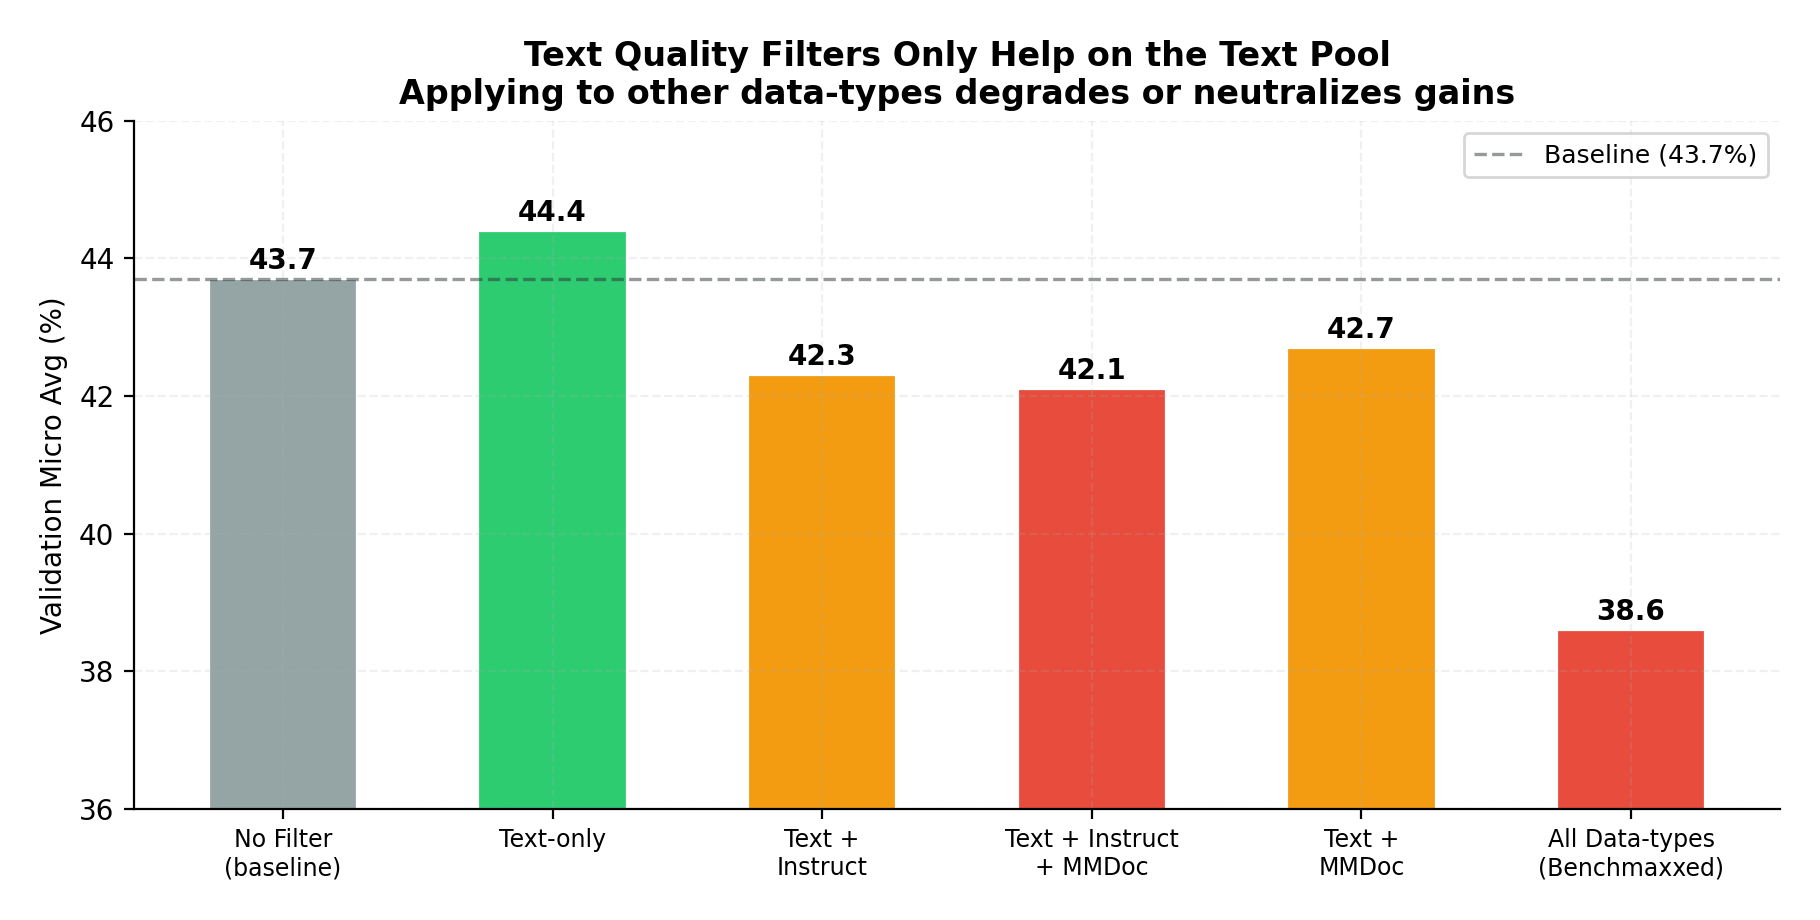
\includegraphics[width=0.9\linewidth]{figures/fig13_filter_dtype_ablation.png}
\caption{\textbf{Text quality filters only help on the text pool.} Extending NVIDIA Mixtral filtering to instruction or multimodal document data types degrades or neutralizes gains. The text data distribution is uniquely amenable to quality-based filtering.}
\label{fig:filter_dtype}
\end{figure}
}


\newcommand{\figlocalrankladder}{%
\begin{figure}
    \centering
    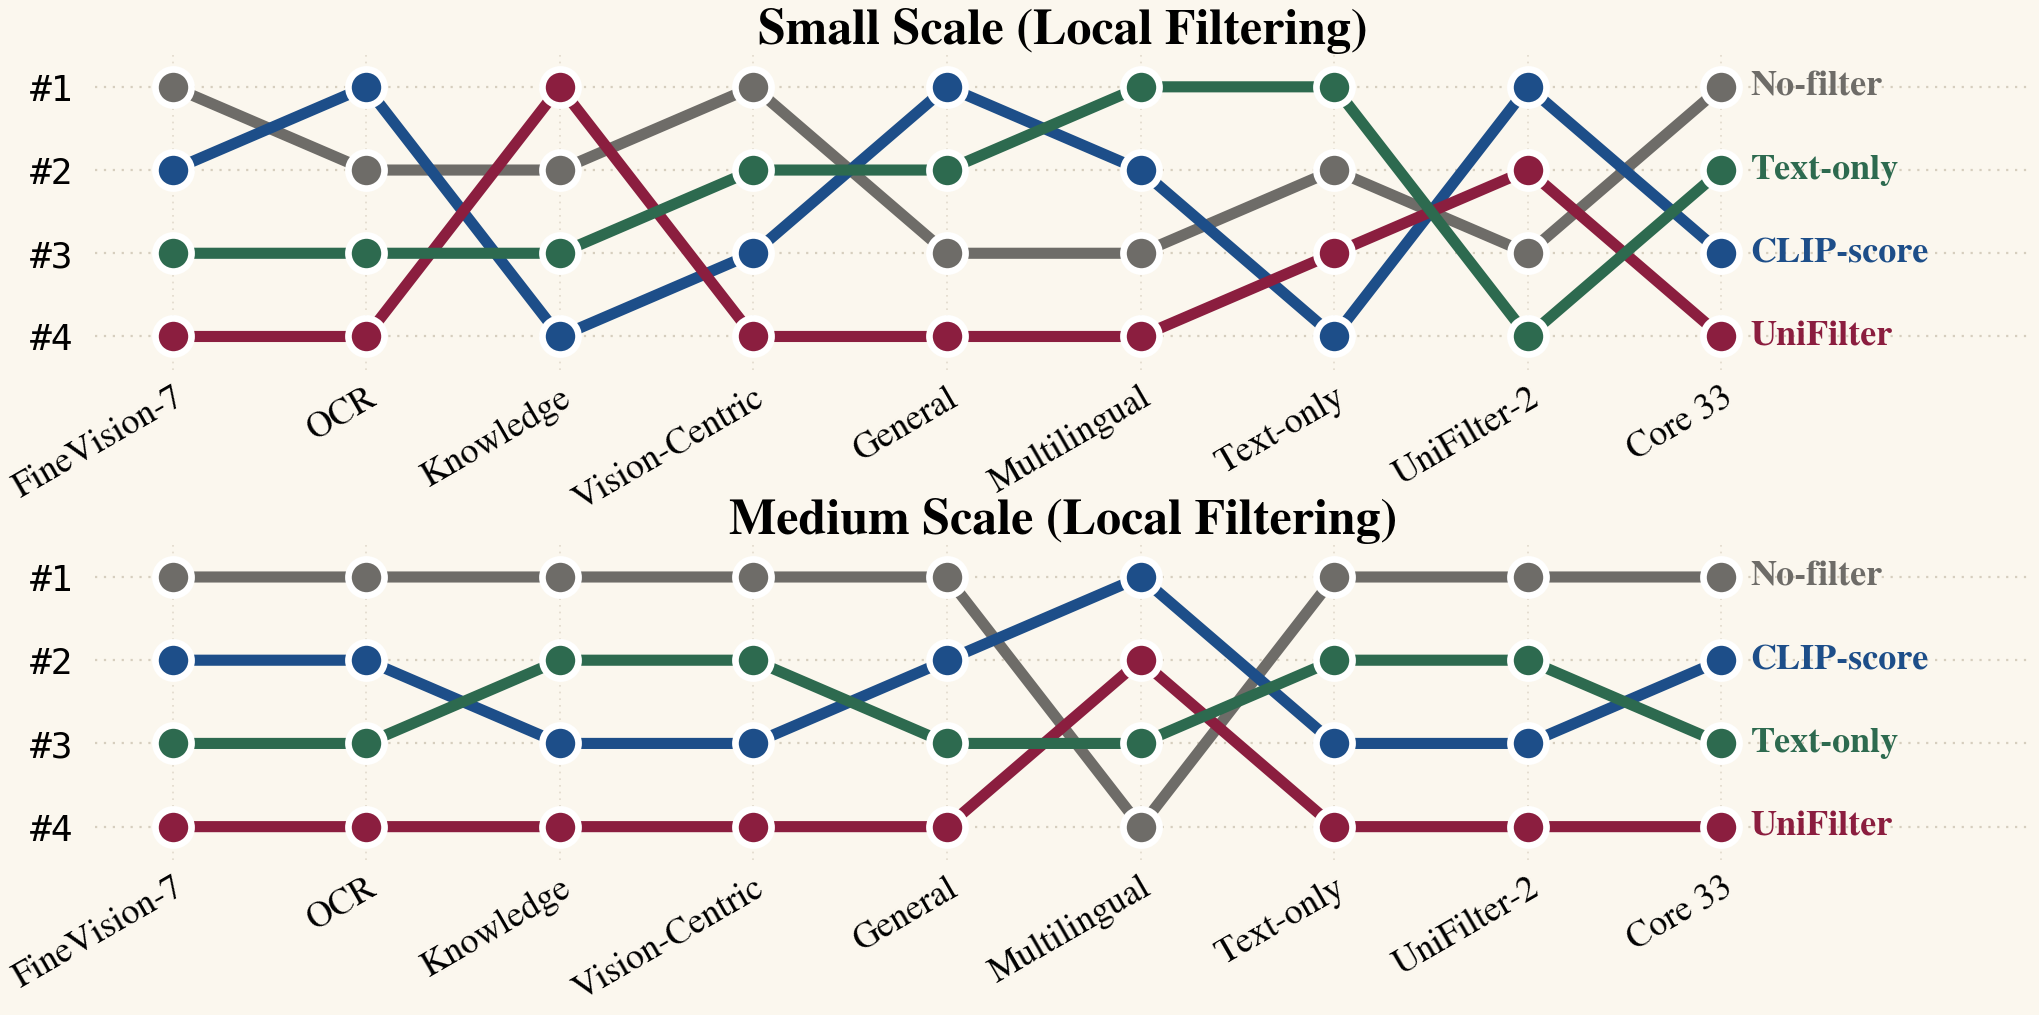
\includegraphics[width=\linewidth]{figures/fig_local_rank_ladders.png}
    \caption{Insert Caption}
    \label{fig:local_rank_ladder}
\end{figure}
}

\newcommand{\figpoolcomposition}{%
\begin{figure}[!h]
\centering
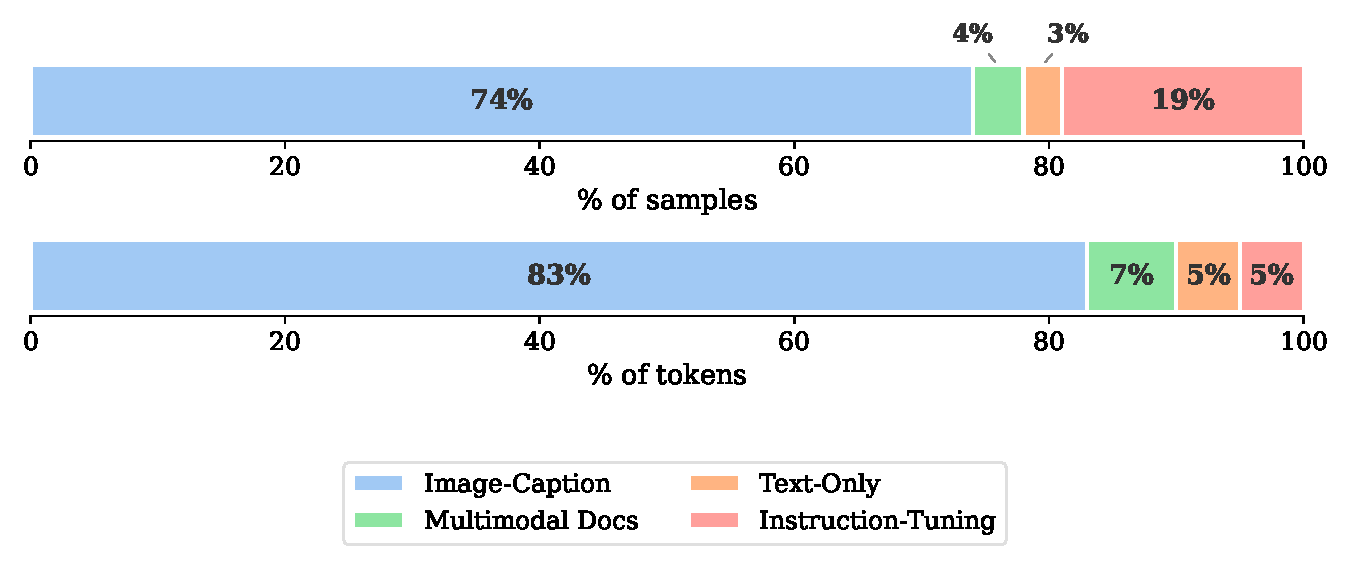
\includegraphics[width=\linewidth]{figures/fig_pie.pdf}
\caption{\textbf{DCVLM pool composition by data type.} Share of total samples (\textit{top}) vs.\ share of total multimodal tokens (\textit{bottom}) for each of the four data types. 
The pool is dominated by image-caption pairs on both axes  (83\% tokens vs\ 74\% samples). Text-only data exhibits the opposite asymmetry, with 19\% of samples but only 5\% of tokens. 
Instruction-tuning data and Multimodal documents are token-dense, i.e, their overall token proportion is much larger than their overall sample proportion, thanks to the presence of potentially many multi-image examples contributing to visual tokens.}
\label{fig:pool-composition}
\end{figure}
}

\newcommand{\figpoolscatter}{%
\begin{figure}[!t]
\centering
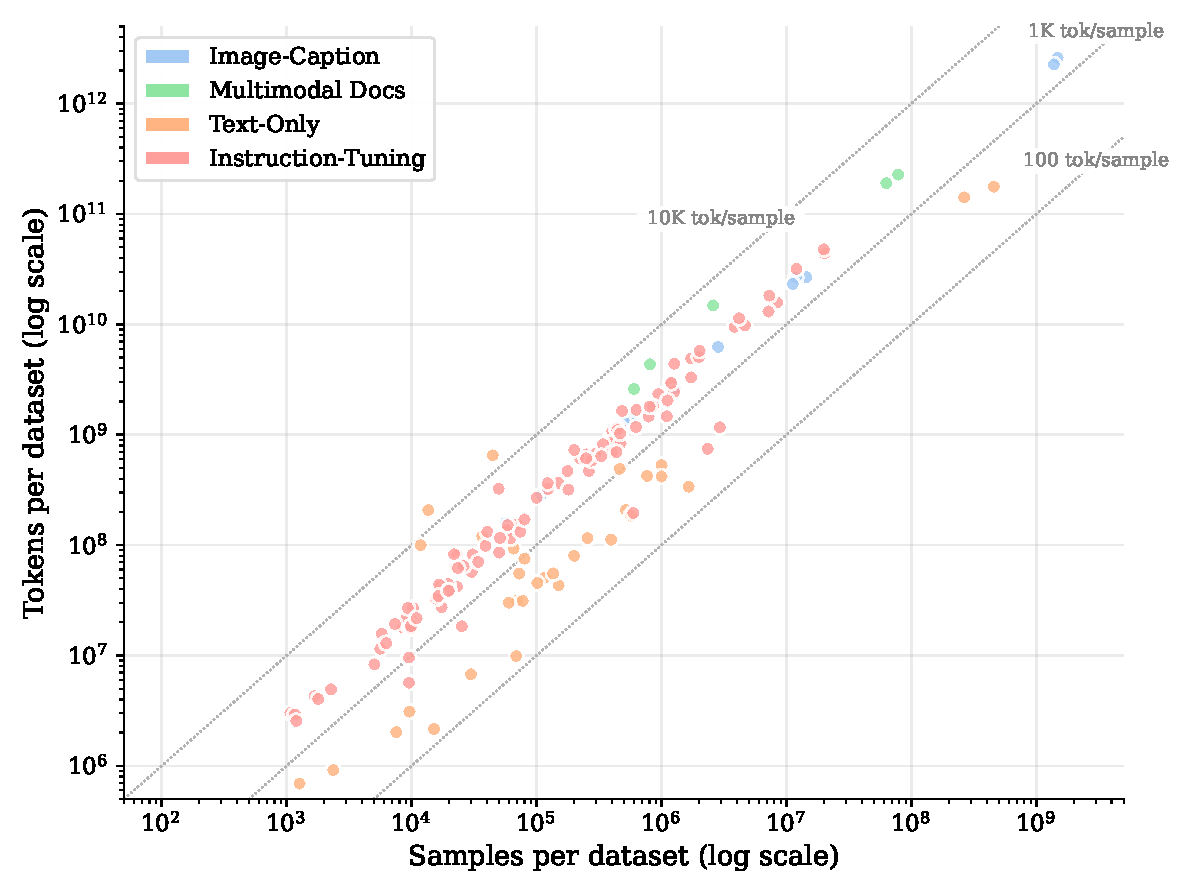
\includegraphics[width=0.78\linewidth]{figures/fig_pool_dataset_scatter.pdf}
\caption{\textbf{Samples vs.\ multimodal tokens (log--log).}
Each marker is one of 160 datasets in our pool, colored by data type.
Diagonal reference lines mark constant tokens-per-sample regimes (100, 1K, 10K).
Image-caption datasets cluster tightly along the 1--2K tok/sample diagonal driven by the visual-token contribution per image; multimodal documents sit one decade higher (multi-image samples); text-only datasets occupy a much wider band (100--15K tok/sample) reflecting the diversity of short instruction data and long-context corpora; instruction-tuning datasets span the largest dynamic range in size (10$^3$--10$^7$ samples) but a relatively narrow tokens-per-sample band.}
\label{fig:pool-scatter}
\end{figure}
}

\newcommand{\figpooltokensper}{%
\begin{figure}[!t]
\centering
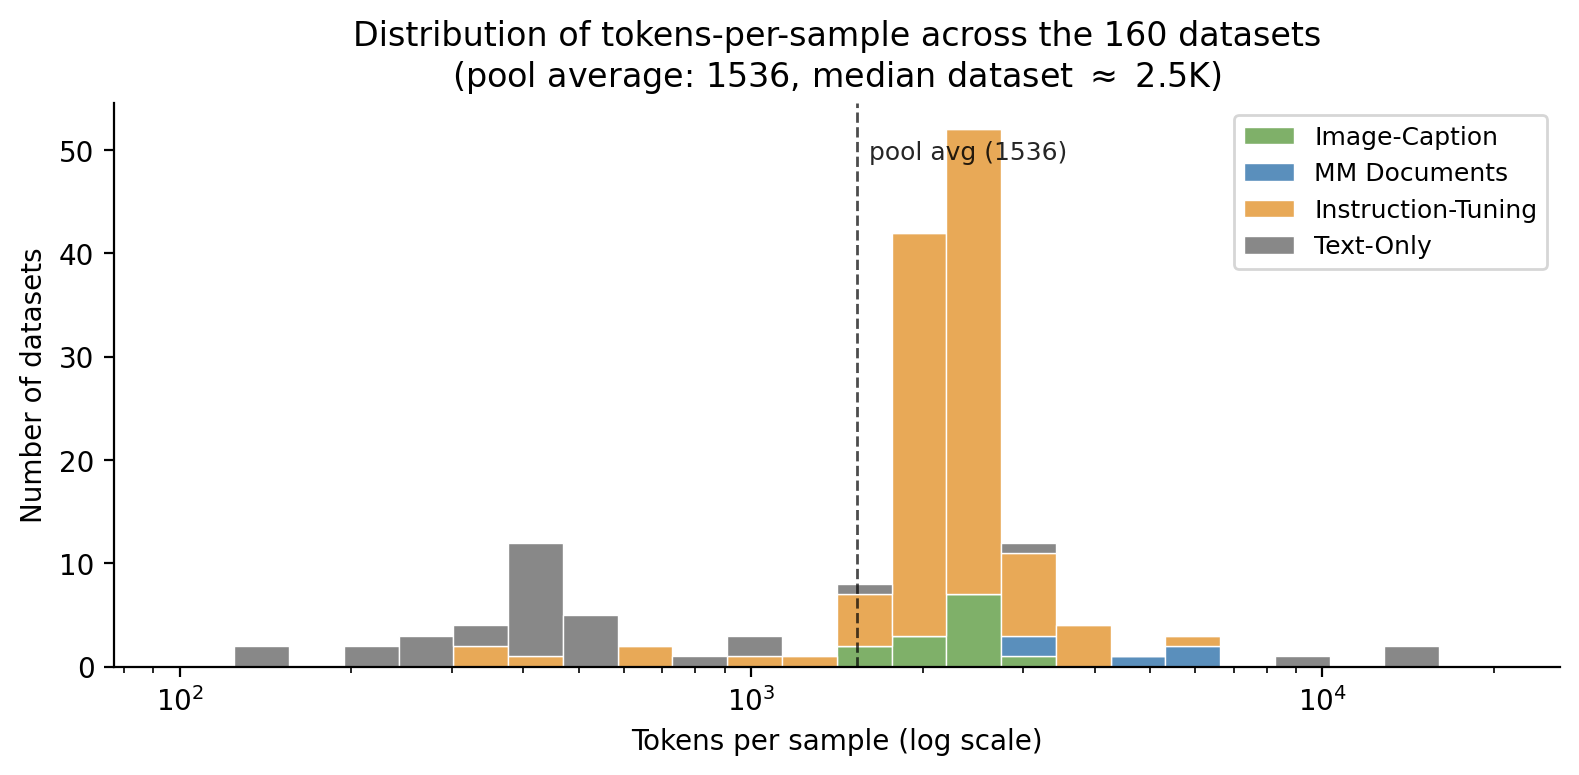
\includegraphics[width=0.85\linewidth]{figures/fig_pool_tokens_per_sample.png}
\caption{\textbf{Distribution of tokens-per-sample across the 160 datasets,} stacked by data type.
The bulk of datasets (128 of 160) fall in the 1K--5K tok/sample range. Text-only datasets dominate the low tail (100--500 tok/sample, short instruction data such as Dolly and Unnatural-Instructions), while a small set of long-context text corpora (LongCite-45K, Long-Instruction-Paraphrase, LongAlpaca) and dense multimodal-document datasets (MINT-PDF, WanJuan) push past 5K tok/sample.}
\label{fig:pool-tokens-per-sample}
\end{figure}
}

\newcommand{\figlangdistribution}{%
\begin{figure}[!t]
\centering
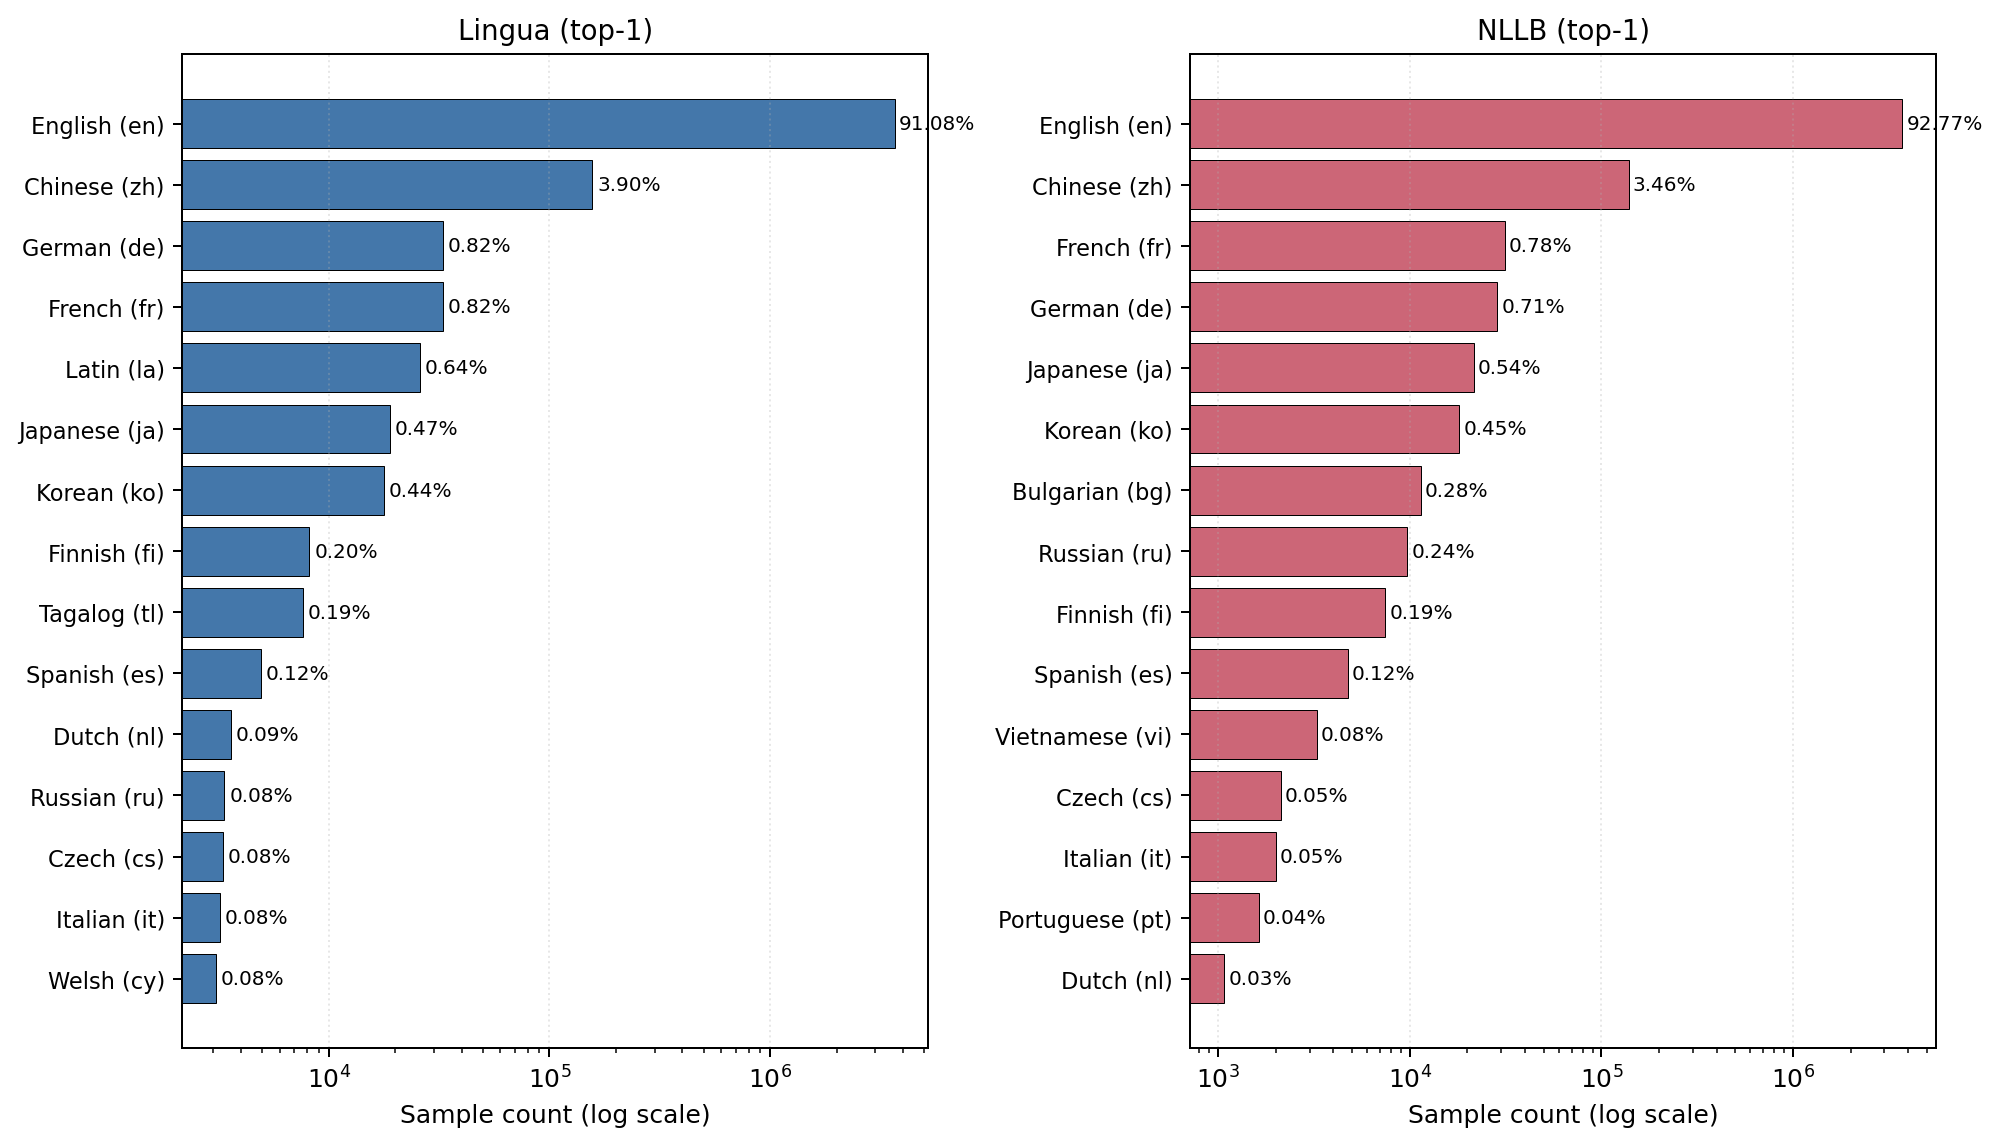
\includegraphics[width=0.95\linewidth]{figures/fig_lang_distribution.png}
\caption{\textbf{Language distribution of \dcvlm{} pool}.
Top-15 languages by per-sample top-1 prediction from \textbf{Lingua} (left, blue) and \textbf{NLLB} (right, red), shown on a log-scaled x-axis.
The pool is dominated by English ($91.1\%$ Lingua / $92.8\%$ NLLB), followed by Chinese ($3.9\%$ / $3.5\%$); the remaining $\sim$5\% is spread across 73 languages (Lingua) or 114 languages (NLLB), with French, German, Japanese, Korean, and Russian forming the next tier.}
\label{fig:lang-distribution}
\end{figure}
}
